\documentclass[12pt,a4paper]{ctexart}

% Language setting
\usepackage[british]{babel}
\addto\captionsbritish{%
  \renewcommand{\abstractname}{摘要}%
  \renewcommand{\figurename}{图}%
  \renewcommand{\tablename}{表}%
}

% Set page size and margins
\usepackage[a4paper,top=2cm,bottom=2cm,left=2.5cm,right=2.5cm,marginparwidth=1.75cm]{geometry}

%----------- APA style references & citations (starting) ---
% Useful packages
%\usepackage[natbibapa]{apacite} % APA-style citations.

\usepackage[style=apa, backend=biber]{biblatex} % APA 7th edition style citations using biblatex
\addbibresource{references.bib} % Your .bib file

% Formatting DOI in APA-7 style
%\renewcommand{\doiprefix}{https://doi.org/}

% Add additional APA 7th edition requirements
\DeclareLanguageMapping{british}{british-apa} % Set language mapping
\DeclareFieldFormat[article]{volume}{\apanum{#1}} % Format volume number

% Modify 'and' to '&' in the bibliography
\renewcommand*{\finalnamedelim}{%
  \ifnumgreater{\value{liststop}}{2}{\finalandcomma}{}%
  \addspace\&\space}

%----------- APA style references & citations (ending) ---


\usepackage{amsmath}
\usepackage{graphicx}
\usepackage{tikz}
\usetikzlibrary{arrows.meta,positioning,calc}
\usepackage[colorlinks=true, allcolors=blue]{hyperref}
\usepackage{hyperref}
%\usepackage{orcidlink}
\usepackage[title]{appendix}
\usepackage{mathrsfs}
\usepackage{amsfonts}
\usepackage{booktabs} % For \toprule, \midrule, \botrule
\usepackage{threeparttable} % For table footnotes
\usepackage{algorithm}
\usepackage{algorithmicx}
\usepackage{algpseudocode}
\usepackage{listings}
\usepackage{enumitem}
\usepackage{chngcntr}
\usepackage{booktabs}
\usepackage{subcaption}
\usepackage{authblk}
\usepackage{csquotes}       % Include csquotes
\usepackage{diagbox}
\usepackage{url}

%\usepackage[justification=raggedright, singlelinecheck=false]{caption}
\usepackage{helvet}  % Load Helvetica (Arial-like)
\usepackage{lmodern}  % Ensures default LaTeX font is available

% label format: capital, centering, and parens
\renewcommand{\thesubfigure}{\Alph{subfigure}}

% Customize line spacing
\usepackage{setspace}
\onehalfspacing % 1.5 line spacing5.3 Discussion and evidence boundaries

% Redefine section and subsection numbering format
\usepackage{titlesec}
\titleformat{\section} % Redefine section numbering format
  {\normalfont\Large\bfseries}{\thesection.}{1em}{}
\titleformat{\subsection}
  {\normalfont\large\bfseries}{\thesubsection}{0.7em}{}

% Customize line numbering format to right-align line numbers
%\usepackage{lineno} % Add the lineno package
%\renewcommand\linenumberfont{\normalfont\scriptsize\sffamily\color{blue}}
%\rightlinenumbers % Right-align line numbers

%\linenumbers % Enable line numbering

% Define a new command for the fourth-level title.
\newcommand{\subsubsubsection}[1]{%
  \vspace{\baselineskip}% Add some space
  \noindent\textbf{#1\\}\quad% Adjust formatting as needed
}
% Change the position of the table caption above the table
\usepackage{float}   % for customizing caption position
\usepackage{caption}
\usepackage{placeins}
\captionsetup[table]{position=top} % caption position for tables
\captionsetup[table]{labelfont=bf} % caption label
\captionsetup[figure]{labelfont=bf} % caption label

% Define the unnumbered list
\makeatletter
\newenvironment{unlist}{%
  \begin{list}{}{%
    \setlength{\labelwidth}{0pt}%
    \setlength{\labelsep}{0pt}%
    \setlength{\leftmargin}{2em}%
    \setlength{\itemindent}{-2em}%
    \setlength{\topsep}{\medskipamount}%
    \setlength{\itemsep}{3pt}%
  }%
}{%
  \end{list}%
}
\makeatother

% Suppress the warning about \@parboxrestore

\date{}  % Remove date


\begin{document}
\renewcommand{\abstractname}{摘要}
\renewcommand{\figurename}{图}
\renewcommand{\tablename}{表}


%----------


\begin{center}
{\Huge 面向完整飞机 B-Rep 模型可追溯小特征识别的面级图学习}
\\[1.5ex]
{\small 中文阅读译本；图片内的英文标注与参考文献题名沿用原稿。}
\\[4ex]

{\large 第一作者} \\
{\small
院系、大学、街道、城市、省州及邮编、国家 \\
first.author@univ.edu \\
\url{https://orcid.org/0000-0002-1010-2288}
} \\[1.2em]

{\large 第二作者} \\
{\small
部门、公司、街道、城市、省州及邮编、国家 \\
second.author@company.com
} \\[1.2em]

{\large 第三作者} \\
{\small
部门、机构、街道、城市、省州及邮编、国家 \\
院系、大学、街道、城市、省州及邮编、国家 \\
third.author@org.org \\
\url{https://orcid.org/0000-0001-1015-3377}
} \\[1.2em]

{\large 第四作者} \\
{\small
部门、研究所、街道、城市、省州及邮编、国家 \\
fourth.author@inst.edu
} \\[1.2em]

{\large 第五作者 \small（通讯作者）} \\
{\small
院系、大学、街道、城市、省州及邮编、国家 \\
user\_id@univ.edu \\
\url{https://orcid.org/0000-0003-1025-5678}
}
\end{center}

\begin{abstract}
  B-Rep 几何特征识别是 CAD 编辑与分析的基础。已有研究广泛关注圆角、倒角和孔等由形状定义的特征。在完整飞机的工业仿真场景中，铆钉面和表面特征面的识别同样重要：在固定弦高偏差容差下，其小半径、边界和局部曲率可能引发局部网格加密，增加三角形数量和网格生成时间。去除这些特征时，仍需保持与可编辑 B-Rep 面的关联，以便进行局部曲面重建，并形成更连续的外表面供网格准备使用。本文提出面向铆钉和表面特征识别的面级图学习框架：每个 B-Rep 面对应一个图节点，共享边界定义邻接关系；两个针对不同类别的图神经网络分别学习铆钉和表面特征的判别函数，每条导出的预测均保留原始 B-Rep 面标识符，以支持分阶段处理和结果检查。在包含 34,162 个面的完整测试集上，铆钉和表面特征的 F1 分数分别为 0.9312 和 0.8091。在固定网格设置下，原始模型与简化模型的配对比较表明，表面三角形数量减少 0.57\%--48.66\%，网格生成时间的中位数减少 2.49\%--58.29\%。这些结果记录了测试条件下的面级识别、可追溯的 CAD 处理候选面及配对网格变化；操作层面的完整性、向其他 CAD 来源的迁移能力和仿真响应保持情况仍需进一步验证。
%\lipsum[1]
\end{abstract}

{\small\textbf{关键词：}B-Rep 可追溯性；图学习；铆钉识别；表面特征；几何处理。}

%-------------------------------------------
% Paper Body
%-------------------------------------------
%--- Section ---%
\section{引言}

完整飞机 B-Rep 模型保留了设计与分析所需的几何实体和拓扑实体，同时也包含大量需要单独检查或处理的局部结构。在本文评估的飞机模型中，铆钉、贴花、窗户及相关表面特征只占少量面，背景面则占绝大多数。识别这些稀少目标时，还必须使每条预测与后续几何操作对应的 CAD 实体保持关联。

传统 CAD 特征识别方法使用几何规则、属性邻接图、分解或基于特征线索的推理来识别制造特征 \parencite{han2000manufacturing,shah2001discourse}。近年来，学习方法直接处理 B-Rep 几何与拓扑，使面级预测不必完全依赖中间网格或点云 \parencite{jayaraman2021uvnet,lambourne2021brepnet,colligan2022hierarchical,wu2024aagnet}。这些研究证明了 B-Rep 表示的价值，但常见研究对象与标签主要是机械零件、建模操作语义或加工特征，而非完整飞机上的铆钉及多样化表面特征。

由于目标面稀少，汇总准确率容易掩盖类别层面的错误 \parencite{he2009learning}。自由曲面以及 B-Rep 面划分方式的差异，也限制了单个面所能提供的信息。当预测用于指导去除或重建时，在大面积平滑背景面上产生的误报可能比漏掉一个局部目标带来更大的几何风险。因此，需要报告逐机错误数、误判背景面的面积，并记录原始面标识符。数据划分以完整飞机为单位，使相关面和局部子图保持在同一集合中 \parencite{kapoor2023leakage}。

本文构建面级图学习与几何处理框架，用于识别完整飞机 B-Rep 模型中的铆钉和其他表面特征。框架将面的几何属性与拓扑属性输入两个针对不同类别的 GNN，将分支分数融合为三类预测，对高风险候选面施加保守的结构约束，并保留预测与面标识符之间的对应关系，以供后续特征去除与局部重建使用。

本文的主要工作包括：
\begin{enumerate}[label=(\arabic*)]
  \item 构建用于三类预测的面级 B-Rep 图表示，类别为\textit{背景}、\textit{铆钉}和\textit{表面特征}。表面特征类包含贴花、窗户等非铆钉的小型表面特征。
  \item 两个类别专用 GNN 分别使用独立参数预测铆钉和表面特征，并按铆钉优先的规则将分数融合为三类标签。
  \item 训练集和测试集按完整飞机划分，而非随机划分面。除汇总分类指标外，评估还报告各机目标类真实面数、漏检面数和 F1，以及背景面误报数和最大相对面积。
  \item 每条预测均保留原始面标识符，使候选面能够在对应的 B-Rep 模型上定位，支持分阶段去除与重建。
  \item 保守的候选面检查限制进入几何处理的预测面，同时逐机报告剩余背景面误报。
\end{enumerate}

%--- Section ---%
\section{相关工作}\label{sec2}

完整飞机 B-Rep 模型的小特征处理主要与两个研究方向相关：三维场景分割和 CAD 特征识别。前者侧重在采样得到的三维数据中定位语义区域或实例区域，后者则在可编辑模型内识别能够支持后续几何操作的实体。对工业 CAD 模型而言，仅获得区域级识别结果不足以直接支持特征去除或重建；结果还必须对应参数化面及其拓扑关系。因此，下文依次讨论三维场景分割、CAD 特征识别，以及下游仿真处理中对小几何结构识别的要求。

\subsection{三维深度学习与场景分割}

三维深度学习已经发展出用于语义分割和实例分割的多种表示，包括体素、点云、多边形网格和多视角图像。PointNet 通过对无序点集学习，为点级分割提供了直接路径 \parencite{qi2017pointnet}。此后的开放词汇方法将图像信息引入重建的三维场景。OpenMask3D 为各三维实例候选融合多个视角的特征；Open3DIS 则将二维实例掩码映射至点云区域，并跨视角合并候选 \parencite{takmaz2023openmask3d,nguyen2024open3dis}。这些方法表明，图像特征和多视角投影能够将识别范围扩展到固定训练标签集合之外。

OpenMask3D 和 Open3DIS 的输出是由重建点云与带位姿的 RGB-D 图像得到的语义区域或实例区域，研究对象通常是室内或其他重建场景 \parencite{takmaz2023openmask3d,nguyen2024open3dis}。这类区域本身并不指向可编辑 CAD 实体中的参数化面或拓扑关系。因此，若将场景分割结果用于局部几何去除，还需要把检测区域重新映射到 B-Rep。CAD 特征识别方法从实体级需求出发，为可编辑模型的操作提供了更直接的起点。

\subsection{从规则到 B-Rep 学习的 CAD 特征识别}

CAD 特征识别研究传统上聚焦于提取制造信息，并支持计算机辅助工艺规划。相关方法使用几何规则、属性邻接图、体分解与重组以及特征线索，识别孔、槽、凸台等局部结构 \parencite{han2000manufacturing,shah2001discourse,babic2008review}。当特征定义和拓扑模板明确时，这些方法具有较好的可解释性。但当特征相互作用、阈值具有领域特异性、曲面为自由形式，或相同设计意图对应不同面划分时，方法迁移会更加困难 \parencite{shah2001discourse}。属性邻接图同时保留面及其拓扑关系，是通向学习式识别的自然桥梁。然而，传统子图匹配仍依赖预定义模式，因而难以适应拓扑变化或特征相互作用。

近期 CAD 学习方法将 B-Rep 实体及其关系保留在学习表示中，不再仅依赖人工设计的模板。UV-Net 将参数化曲面、曲线信息与邻接图拓扑结合；BRepNet 则在面、边和有向共边之间传递消息，用于建模操作分割 \parencite{jayaraman2021uvnet,lambourne2021brepnet}。Hierarchical CADNet 在 B-Rep 面邻接图之外加入表面网格层和边的凸性，用于加工特征识别；AAGNet 研究了属性邻接图上的多任务加工特征识别 \parencite{colligan2022hierarchical,wu2024aagnet}。这些研究展示了将 B-Rep 几何与拓扑提供给面级学习的多种有效方式。不过，它们的数据集和标签主要面向机械零件、合成 CAD 集合、建模操作语义或加工特征，与本文区分完整飞机模型中\textit{背景}面、\textit{铆钉}面和多样化\textit{表面特征}面的任务有所不同。

\subsection{工业仿真流程中的小几何结构识别需求}

在工业仿真流程中，局部特征识别只是中间步骤：识别结果可能决定网格生成和分析前保留、去除或重建该特征。CAD 简化与考虑分析需求的特征去除研究探讨了特征去除的几何后果 \parencite{thakur2009cad_simplification,antolin2024analysis_aware_defeaturing}；B-Rep 学习研究表明，面级预测可以与源实体保持关联 \parencite{jayaraman2021uvnet,lambourne2021brepnet,yeo2021machining}。这两个方向分别满足互补需求，但现有文献对这样一条路径的记录仍有限：在完整工业模型上识别小而多样的局部几何结构，并将面级预测转化为可追溯的 CAD 处理候选面。

汇总分割准确率无法指出哪些背景面可能被错误修改。例如，大面积平滑壳体面上的误报，对后续几何处理的影响可能大于漏掉一个局部目标。因此，本文采用 B-Rep 面级任务表述，将面标识符传递到处理阶段，并逐机报告错误。下文的表示方式正是基于这一要求：以面作为图节点，以共享边界提供局部上下文，并用面标识符维持预测与 CAD 实体之间的联系。


%--- Section ---%
\section{B-Rep 基础与图学习}\label{sec:methods}

\subsection{B-Rep 基础}\label{sec:brep_preliminary}

边界表示（B-Rep）通过将顶点、边、线环（或闭合环）、面、壳和实体等拓扑实体与其底层几何实体关联来描述三维实体 \parencite{iso10303_42_2025}。面通常以参数化曲面为支撑，并由一个外环及可能存在的内环裁剪为有限的可见区域。裁剪边界可以是解析曲线或 B 样条曲线，支撑曲面也可以是 B 样条曲面。因此，相邻面即使位于相似的曲面上，也可能具有不同的裁剪环和邻接关系。B-Rep 保留了这些关系；若模型被降为无结构点集，则无法直接获取它们。这些信息使每条预测既可作为学习目标，也可指向可定位的 CAD 实体。图~\ref{fig:brep_preliminary} 展示了这一含义。

\begin{figure}[!ht]
\centering
\begin{tikzpicture}[
  font=\sffamily\scriptsize,
  >=Latex,
  entity/.style={font=\sffamily\bfseries\small, text=black!85},
  outline/.style={draw=black!78, line width=.65pt, line join=round},
  hidden/.style={draw=black!55, line width=.55pt, dashed}
]
  % Body, shell, face, loop, edge, and vertex are shown as peer B-Rep entities.
  \node[entity] at (-5.55,2.45) {实体};
  \path[fill=black!6, draw=black!78, line width=.65pt] (-6.70,.52) -- (-6.70,1.67)
    .. controls (-6.15,1.98) and (-5.58,1.94) .. (-5.28,1.53) -- (-5.28,.52) -- cycle;
  \path[fill=blue!16, draw=blue!70!black, line width=.65pt] (-6.70,1.67)
    .. controls (-6.15,1.98) and (-5.58,1.94) .. (-5.28,1.53)
    -- (-4.96,1.75) .. controls (-5.25,2.16) and (-5.85,2.22) .. (-6.38,1.89) -- cycle;
  \path[fill=black!3, draw=black!78, line width=.65pt] (-5.28,.52) -- (-4.96,.74) -- (-4.96,1.75) -- (-5.28,1.53) -- cycle;
  \draw[hidden] (-6.70,.52) -- (-6.38,.74) -- (-4.96,.74);

  \node[entity] at (-2.75,2.45) {壳};
  % The same curved boundary as the body, with its faces slightly separated.
  \path[fill=black!6, draw=black!78, line width=.65pt] (-3.93,.49) -- (-3.93,1.64)
    .. controls (-3.38,1.95) and (-2.81,1.91) .. (-2.51,1.50) -- (-2.51,.49) -- cycle;
  \path[fill=blue!20, draw=blue!70!black, line width=.65pt] (-3.90,1.76)
    .. controls (-3.35,2.07) and (-2.78,2.03) .. (-2.48,1.62)
    -- (-2.16,1.84) .. controls (-2.45,2.25) and (-3.05,2.31) .. (-3.58,1.98) -- cycle;
  \path[fill=black!3, draw=black!78, line width=.65pt] (-2.42,.52) -- (-2.10,.74) -- (-2.10,1.75) -- (-2.42,1.53) -- cycle;
  \draw[hidden] (-3.93,.49) -- (-3.61,.71) -- (-2.10,.74);

  \node[entity] at (.00,2.45) {面};
  \path[fill=blue!20, draw=blue!70!black, line width=.7pt] (-.68,.67)
    .. controls (-.53,1.28) and (-.02,1.55) .. (.62,1.40)
    -- (.51,.75) .. controls (-.02,.61) and (-.38,.56) .. (-.68,.67) -- cycle;

  \node[entity] at (2.60,2.45) {环};
  \draw[outline] (1.76,.65) .. controls (1.94,1.27) and (2.48,1.59) .. (3.20,1.42)
    -- (3.08,.72) .. controls (2.44,.55) and (2.02,.54) .. (1.76,.65) -- cycle;
  \draw[draw=blue!70!black, line width=1.05pt] (1.76,.65)
    .. controls (1.94,1.27) and (2.48,1.59) .. (3.20,1.42);
  \foreach \p in {(1.76,.65),(3.20,1.42),(3.08,.72)}
    {\filldraw[fill=white, draw=black!75] \p circle (1.05pt);}

  \node[entity] at (4.88,2.45) {边};
  \draw[draw=blue!70!black, line width=1.05pt] (4.15,.78)
    .. controls (4.55,1.40) and (5.12,1.58) .. (5.62,1.23);
  \filldraw[fill=white, draw=blue!70!black] (4.15,.78) circle (1.05pt);
  \filldraw[fill=white, draw=blue!70!black] (5.62,1.23) circle (1.05pt);
  \draw[-{Latex[length=1.5mm]}, draw=blue!65!black, line width=.6pt] (3.45,1.08) -- (3.92,1.08);

  \node[entity] at (6.75,2.45) {顶点};
  \filldraw[fill=black!78, draw=black!80] (6.75,1.02) circle (2.1pt);

\end{tikzpicture}
\caption{曲面 B-Rep 示例中的拓扑实体。为便于比较，实体与壳表示相同的曲面边界：实体合并显示，壳的组成面则用细缝分隔。实体和壳中的蓝色面被单独示出，其边界由环、边和顶点构成；高亮的蓝色环段另以蓝色边表示。}\label{fig:brep_preliminary}
\end{figure}
\FloatBarrier

\subsection{面级监督学习任务}\label{sec:data_preparation}

本文将“小几何结构”仅作为监督学习任务的操作性称谓，而非特征识别规则。标注协议将每个原始 B-Rep 面归入\textit{背景}、\textit{铆钉}或\textit{表面特征}；其中，表面特征包含后续简化或重建中考虑的贴花、窗户等非铆钉目标。类别由标注记录给出，并非根据固定面积、曲率或拓扑模板推断。具体标注过程及模型级划分见第~\ref{sec:data_partition} 节。

对完整飞机 B-Rep，学习目标是在保留面标识符的同时，为每个原始面 $v_i$ 指定背景、铆钉或表面特征三类之一。预测类别及分数与该面标识符一同导出，以便同真实标签对齐、在源模型上检查，并传递到后续几何处理。去除操作产生的中间模型具有新的面标识符集合，因此在第~\ref{sec:geometry_protocol} 节的分阶段流程中单独处理。

\subsection{面图与输入属性}\label{sec:face_graph}

对每个完整飞机 B-Rep 模型，本文构建图 $G=(V,E)$。其中，节点 $v_i\in V$ 表示一个原始面，并保留其面标识符；集合 $E$ 中的边表示共享边界。节点属性描述单个面，边属性描述面之间的关系。面级表示借鉴已有 B-Rep 学习研究 \parencite{yeo2021machining,zhang2024brep2seq}；本文的标签与评估设置则针对第~\ref{sec:data_preparation} 节定义的飞机任务。

图~\ref{fig:face_graph_attributes} 展示相邻面如何成为由共享边界连接的图节点。颜色用于区分不同面，并不代表预测类别。所得图为第~\ref{sec:dual_gnn} 节的类别专用 GNN 提供每个节点 48 个属性和每条图边 6 个属性。

\begin{figure}[!ht]
\centering
\resizebox{\linewidth}{!}{%
\begin{tikzpicture}[
  font=\sffamily\footnotesize,
  flow/.style={-{Latex[length=2.5mm]}, line width=1.15pt, draw=blue!62!black},
  note/.style={align=center, text=black!70, font=\sffamily\scriptsize},
  face/.style={draw=black!62, line width=.7pt},
  card/.style={rounded corners=5pt, inner sep=4.2pt, align=center, font=\sffamily\footnotesize}
]
  \node[font=\sffamily\bfseries\small, text=blue!62!black] at (1.70,1.62) {B-Rep 局部邻域};
  \draw[face, fill=cyan!25] (.28,.06) -- (1.23,.92) -- (2.05,.40) -- (1.66,-.57) -- cycle;
  \draw[face, fill=orange!36] (2.05,.40) -- (3.00,1.00) -- (3.30,-.04) -- (2.47,-.65) -- (1.66,-.57) -- cycle;
  \draw[face, fill=green!28] (.28,.06) -- (1.66,-.57) -- (1.45,-1.10) -- (.76,-1.29) -- cycle;
  \draw[face, fill=blue!35] (1.66,-.57) -- (2.47,-.65) -- (2.20,-1.44) -- (1.45,-1.10) -- cycle;
  \draw[face, fill=violet!22] (2.47,-.65) -- (3.30,-.04) -- (3.72,-1.02) -- (2.20,-1.44) -- cycle;
  \draw[dashed, black!38, line width=.6pt] (1.23,.92) -- (.76,-1.29);
  \node[note] at (1.95,-1.93) {原始面及面标识符};

  \draw[flow] (4.02,-.08) -- (4.82,-.08);

  \node[font=\sffamily\bfseries\small, text=blue!62!black] at (5.90,1.62) {面级图};
  \draw[line width=1pt, black!58] (4.92,.32) -- (5.95,.90) -- (7.15,.35) -- (6.65,-1.10) -- (5.30,-.85) -- (4.92,.32);
  \draw[line width=1pt, black!58] (5.95,.90) -- (6.65,-1.10);
  \foreach \x/\y/\c in {4.92/.32/cyan!72,5.95/.90/orange!80,7.15/.35/violet!66,6.65/-1.10/blue!62,5.30/-.85/green!67} {
    \filldraw[fill=\c, draw=black!65, line width=.55pt] (\x,\y) circle (3.0pt);
  }
  \node[note] at (6.10,-1.93) {$v_i$：面 \quad $e_{ij}$：共享边界};

  \node[draw=blue!60!black, fill=blue!3, rounded corners=5pt, text width=27mm, inner sep=2.6pt, align=left, font=\sffamily\footnotesize] (attributes) at (9.35,-.08) {\textcolor{teal!65!black}{\textbf{节点}}\hfill $\mathbf{x}_i\in\mathbb{R}^{48}$\\[-1pt]\textcolor{black!25}{\rule{26mm}{.25pt}}\\[-1pt]\textcolor{orange!80!black}{\textbf{边}}\hfill $\mathbf{e}_{ij}\in\mathbb{R}^{6}$};
  \draw[flow] (7.38,-.08) -- (attributes.west);

  \draw[flow] (attributes.east) -- (11.40,-.08);
  \node[font=\sffamily\bfseries\small, text=blue!62!black] at (12.62,1.62) {邻域聚合};
  \fill[blue!10] (13.19,-1.10) circle (8.0pt);
  \draw[line width=1pt, black!56] (11.46,.32) -- (12.49,.90) -- (13.69,.35) -- (13.19,-1.10) -- (11.84,-.85) -- (11.46,.32);
  \draw[line width=1pt, black!56] (12.49,.90) -- (13.19,-1.10);
  \foreach \x/\y/\c in {11.46/.32/cyan!70,12.49/.90/orange!77,13.69/.35/violet!63,11.84/-.85/green!66} {
    \filldraw[fill=\c, draw=black!65, line width=.55pt] (\x,\y) circle (2.8pt);
  }
  \draw[-{Latex[length=1.8mm]}, draw=blue!70!black, line width=.75pt] (12.60,.43) -- (13.05,-.82);
  \draw[-{Latex[length=1.8mm]}, draw=blue!70!black, line width=.75pt] (12.17,-.92) -- (12.96,-1.04);
  \draw[-{Latex[length=1.8mm]}, draw=blue!70!black, line width=.75pt] (13.57,.05) -- (13.30,-.82);
  \filldraw[fill=blue!70, draw=blue!70!black, line width=.8pt] (13.19,-1.10) circle (3.7pt);
  \node[note] at (12.60,-1.93) {邻域消息聚合为\\高亮面的表示};

  \draw[flow] (14.22,-.08) -- (14.58,-.08);
  \node[draw=blue!60!black, fill=blue!4, rounded corners=5pt, minimum width=24mm, inner sep=4.2pt, align=center, font=\sffamily\footnotesize, text=blue!62!black] at (15.82,-.08) {类别专用 GNN\\第~\ref{sec:dual_gnn} 节};
\end{tikzpicture}%
}
\caption{从局部 B-Rep 邻域到带属性的面级图。每个原始面成为一个图节点，并保留其面标识符；两个面之间的共享边界成为一条图边。节点属性描述单个面，边属性描述面间关系，两者均参与消息传递。示意图中的颜色仅区分相邻 B-Rep 面，不表示预测类别。}\label{fig:face_graph_attributes}
\end{figure}

当前实现为每个 B-Rep 面设置 48 个节点属性。这些属性按信息来源组织，而非作为手工制定的识别规则：面尺度与形状包括相对面积、周长、紧致度及与邻接面面积的关系；曲面信息包括曲率、半径是否可用及曲面类型；边界组织包括线环、内环和边的数量；局部邻域统计描述相邻曲面类型、凸凹或平滑关系、法向相似性及同曲面连通性。此外，还包括按模型尺度归一化的几何量和相对位置描述量。所得向量刻画 B-Rep 面的局部状态，但单一面积、曲面类型或曲率值均不直接规定其铆钉或表面特征标签。

铆钉通常具有重复的局部形态，而表面特征实例在尺度、曲面形态和附着方式上有所差异。因此，单独使用面面积或曲面类型不能形成可靠的类别规则。飞机模型的物理尺度和面划分也各不相同；若不进行归一化，几何量可能主要反映模型尺寸或导出约定。本文对需要尺度一致性的量进行归一化，并复用训练集计算得到的特征顺序与统计量。第~\ref{sec:results} 节的评估检验的是固定飞机划分上的这一表示，而非任意 CAD 来源。

每个面邻接关系对应六个边属性：连接类型、面积比、邻面曲面类型、共享边长度、平均二面角以及二面角标准差。这些属性描述两个 B-Rep 面之间的边界关系，而不是孤立地描述某一个面。例如，共享边长度反映邻接关系的局部尺度；二面角统计量描述局部转折或连续性；邻面曲面类型和面积比则提供单个节点不具备的关系信息。边条件图卷积的滤波器可受边标签调节，因此为邻域聚合时保留此类信息提供了通用基础 \parencite{simonovsky2017dynamic}。据此，本文在消息传递中提供边属性；类别专用编码器及其学习得到的边条件操作见第~\ref{sec:class_specific_learning} 节。

消息传递将每个面的属性与邻接面及其共享边界的属性结合起来。当单个面的面积、曲率或曲面类型存在歧义时，这种方式提供局部几何和拓扑上下文。如第~\ref{sec:dual_gnn} 节所述，两个类别专用分支接收同一图输入，但分别学习不同的表示。

图节点在张量运算中可以使用连续索引，但导出时每条预测仍对应回原始面标识符。这样，面级标签便可与标注比较、在原始 B-Rep 模型上可视化，并传递至几何处理。三个类别标签定义预测目标；节点和边属性构成学习输入。

\subsection{类别专用图学习}\label{sec:class_specific_learning}

\subsubsection{网络结构与决策融合}\label{sec:dual_gnn}

分类器包含铆钉分支和表面特征分支。两者接收同一个图输入，但各自具有独立的节点编码器、边编码器、图卷积层、适配器和输出头。每个分支学习目标类与背景类之间的二元判别，再将两个分数融合为三类输出。独立参数使两个分支能够学习不同的模式。

图~\ref{fig:class_specific_gnn} 展示两个分支、分数融合以及面标识符的可追溯路径。面标识符将图节点与导出预测连接起来，但不作为神经网络的输入特征。

\begin{figure}[!ht]
\centering
% Exact face-to-node correspondence for the input panel of Figure 3.
% The unchanged raster underneath supplies the two GNN branches and fusion path.
\begingroup
\newdimen\figthreeunit
\figthreeunit=\dimexpr\linewidth/1250\relax
\begin{tikzpicture}[x=\figthreeunit,y=\figthreeunit]
  \node[anchor=south west,inner sep=0,outer sep=0] at (0,0)
    {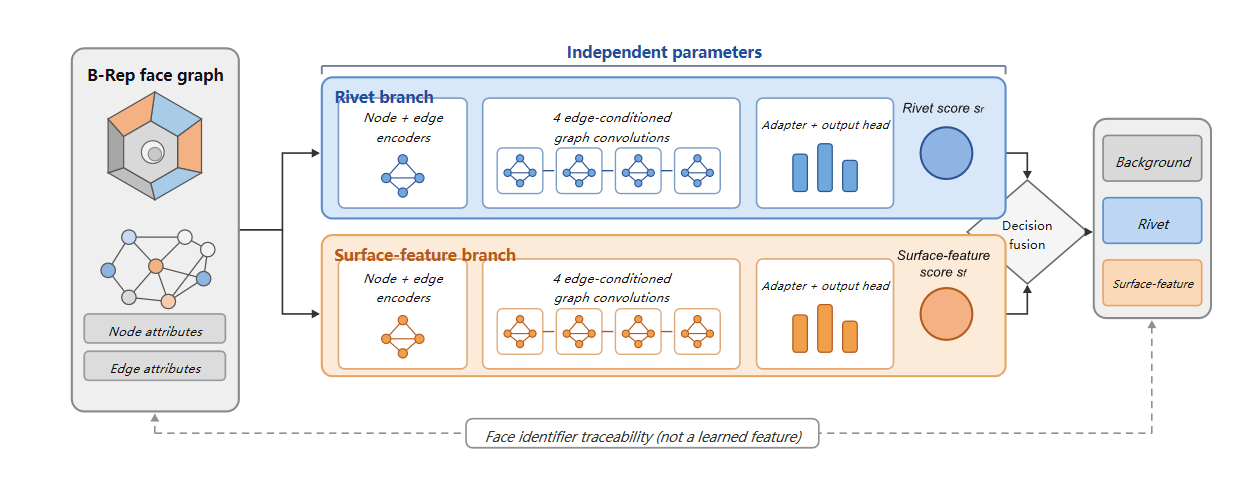
\includegraphics[width=\linewidth]{figures/fig_class_specific_gnn_architecture_v3.png}};

  % Replace only the input panel. A shared B-Rep edge becomes one graph edge.
  \begin{scope}[yshift=34\figthreeunit]
  \path[fill=white] (69,45) rectangle (241,415);
  \draw[rounded corners=13,fill=gray!9,draw=gray!55,line width=1.5\figthreeunit]
    (71,48) rectangle (239,412);
  \node[font=\sffamily\bfseries\fontsize{6.6}{7.5}\selectfont] at (155,389)
    {B-Rep face graph};

  % Four faces of a local B-Rep surface patch, viewed obliquely.
  \path[fill=blue!22,draw=gray!65,line width=1.1\figthreeunit]
    (101,351)--(153,366)--(151,322)--(101,308)--cycle;
  \path[fill=orange!38,draw=gray!65,line width=1.1\figthreeunit]
    (153,366)--(209,349)--(209,305)--(151,322)--cycle;
  \path[fill=gray!35,draw=gray!65,line width=1.1\figthreeunit]
    (101,308)--(151,322)--(151,280)--(101,265)--cycle;
  \path[fill=blue!46,draw=gray!65,line width=1.1\figthreeunit]
    (151,322)--(209,305)--(209,264)--(151,280)--cycle;
  \draw[draw=blue!75!black,line width=2.5\figthreeunit]
    (153,366)--(151,322);
  \node[font=\sffamily\bfseries\fontsize{6.3}{7}\selectfont] at (127,338) {F1};
  \node[font=\sffamily\bfseries\fontsize{6.3}{7}\selectfont] at (181,337) {F2};
  \node[font=\sffamily\bfseries\fontsize{6.3}{7}\selectfont] at (127,294) {F3};
  \node[font=\sffamily\bfseries\fontsize{6.3}{7}\selectfont] at (181,292) {F4};

  \node[font=\sffamily\fontsize{5.3}{6}\selectfont,text=black!70]
    at (155,245) {Shared edge $\rightarrow$ link};

  % F1--F4 and F2--F3 meet only at a vertex, so no diagonal graph edge exists.
  \draw[draw=gray!70,line width=1.2\figthreeunit] (121,214)--(121,166);
  \draw[draw=gray!70,line width=1.2\figthreeunit] (188,214)--(188,166);
  \draw[draw=gray!70,line width=1.2\figthreeunit] (121,166)--(188,166);
  \draw[draw=blue!75!black,line width=2.5\figthreeunit] (121,214)--(188,214);
  \foreach \x/\y/\name/\colour in {
    121/214/F1/blue!22,
    188/214/F2/orange!38,
    121/166/F3/gray!35,
    188/166/F4/blue!46
  } {
    \node[circle,minimum size=27\figthreeunit,inner sep=0,
      draw=gray!70,fill=\colour,line width=1.2\figthreeunit,
      font=\sffamily\bfseries\fontsize{5.8}{6.5}\selectfont]
      at (\x,\y) {\name};
  }

  \draw[rounded corners=4,fill=gray!16,draw=gray!55,line width=1.1\figthreeunit]
    (84,116) rectangle (226,145);
  \node[font=\sffamily\itshape\fontsize{5.6}{6.5}\selectfont]
    at (155,130) {Node attributes};
  \draw[rounded corners=4,fill=gray!16,draw=gray!55,line width=1.1\figthreeunit]
    (84,80) rectangle (226,109);
  \node[font=\sffamily\itshape\fontsize{5.6}{6.5}\selectfont]
    at (155,94) {Edge attributes};
  \end{scope}
\end{tikzpicture}
\endgroup

\caption{具有面标识符可追溯性的面级三类预测网络。相同的 B-Rep 面图、节点属性和边属性进入参数独立的铆钉分支与表面特征分支。每个分支包含独立的属性编码器、四层带残差连接的边条件图卷积、一个适配器和一个输出头。两个 sigmoid 分数按照铆钉优先规则融合，得到背景、铆钉或表面特征标签。虚线表示原始面实体与导出预测之间的可追溯路径，而非学习特征。}
\label{fig:class_specific_gnn}
\end{figure}

对类别专用分支 $k\in\{r,s\}$，其中 $r$ 表示铆钉、$s$ 表示表面特征，原始节点属性和边属性首先由独立编码器变换：
\begin{equation}
\mathbf{h}_{i,k}^{(0)}=\phi_{x,k}(\mathbf{x}_i), \qquad
\tilde{\mathbf{e}}_{ij,k}=\phi_{e,k}(\mathbf{e}_{ij}).
\label{eq:class_specific_input_encoding}
\end{equation}
其中，$\mathbf{x}_i$ 是 B-Rep 面节点 $v_i$ 的 48 维属性向量，$\mathbf{e}_{ij}$ 是面 $i$ 与面 $j$ 邻接关系的 6 维属性向量；$\phi_{x,k}$ 和 $\phi_{e,k}$ 分别是类别专用的节点编码器和边编码器。每个编码器由线性变换、LayerNorm 和 ReLU 激活构成。两个分支的输入属性相同，但 $\phi_{x,r}$、$\phi_{e,r}$、$\phi_{x,s}$ 和 $\phi_{e,s}$ 的参数互不共享。

每个分支使用四层带残差连接的边条件图卷积，隐藏维度为 64。在第 $\ell$ 层，编码后的边属性调节 \texttt{NNConv} 使用的消息变换：
\begin{equation}
\mathbf{u}_{i,k}^{(\ell+1)}=
\operatorname{Dropout}\!\left(
\operatorname{ReLU}\!\left(
\operatorname{LN}\!\left(
\operatorname{NNConv}_{k}
(\mathbf{h}_{i,k}^{(\ell)},\tilde{\mathbf{e}}_{ij,k})
\right)\right)\right).
\label{eq:class_specific_message_update}
\end{equation}
残差连接在感受野扩展时保留节点状态。经过四层后，将局部表示与池化得到的完整飞机上下文拼接，经类别专用适配器映射后送入输出头。边条件滤波使消息变换受边标签调节 \parencite{simonovsky2017dynamic}；本文所用属性、分支和决策规则则面向具体应用。

设 $\mathbf{z}_{i,r}$ 和 $\mathbf{z}_{i,s}$ 为面 $i$ 的两个类别专用表示，其独立 sigmoid 分数为
\begin{equation}
p_{r,i}=\sigma(g_r(\mathbf{z}_{i,r})), \quad
p_{s,i}=\sigma(g_s(\mathbf{z}_{i,s})),
\label{eq:class_specific_scores}
\end{equation}
其中 $g_r$ 和 $g_s$ 为输出头。两个分数按铆钉优先规则转换为最终面标签：
\begin{equation}
\hat{y}_i =
\begin{cases}
\text{铆钉}, & p_{r,i} \geq \tau_r, \\
\text{表面特征}, & p_{r,i} < \tau_r \ \text{且} \ p_{s,i} \geq \tau_s, \\
\text{背景}, & \text{其他情况},
\end{cases}
\label{eq:dual_head_decision}
\end{equation}
其中 $\hat{y}_i$ 是最终类别。固定推理配置使用 $\tau_r=0.9$ 和 $\tau_s=0.5$；表面特征分数不会覆盖已作出的铆钉判定。与模型配套的统计文件保存了这些阈值及特征处理约定。

\subsubsection{学习目标与推理决策}\label{sec:training_inference}

两个分支在相同的完整飞机图上联合优化，对应“背景--铆钉”和“背景--表面特征”两个二元任务。每个输出头使用类别感知的 focal loss（$\gamma=2.0$），以减弱大量已被正确分类的背景面在训练中的主导作用，而不在预测后额外加入手工类别判定规则 \parencite{lin2017focal,buda2018imbalance}。推理时复用保存的特征列顺序和归一化统计量；导出的面标识符、最终类别和分支分数维持与原始 B-Rep 面的联系。第~\ref{sec:processing_pipeline} 节据此定义预测进入几何操作的条件。

\section{特征处理与训练方案}\label{sec:processing_pipeline}

\subsection{保守的候选面筛选}\label{sec:risk_filtering}

保守的后处理只检查被预测为目标类的面，并将被拒绝的候选面恢复为\textit{背景}；它不会将背景预测提升为目标类。当预测铆钉面的相对面积超过 $5\times10^{-6}$ 时，铆钉检查会拒绝该预测。表面特征检查根据面几何和局部邻接关系拒绝特定的机翼或壳体拓扑；在原始模型的表面特征阶段，若候选面的采样点沿六个笛卡尔坐标方向均不存在无遮挡射线，外部可见性检查也会拒绝该候选面。报告的面级识别标签还经过平面区域铆钉检查和一轮表面特征筛选；仅处理贴花的路线则使用单独的拓扑检查。这些检查定义了报告的标签和处理候选面，但并不测量几何操作的成功情况。

\subsection{分阶段去除、重建与验证}\label{sec:geometry_protocol}

每个保留的候选面都携带其预测所依据的 B-Rep 模型中的面标识符。处理阶段利用该标识符定位面、执行去除或局部重建，并保留与输入模型之间可核查的联系。不过，预测准确性、操作成功与否以及是否适合特定工程分析，仍需分别检查；能否用于仿真取决于任务、载荷、边界条件及必须保持完整的区域 \parencite{thakur2009cad_simplification,antolin2024analysis_aware_defeaturing}。

去除或重建会改变拓扑和面编号。因此，一个面标识符只能在产生该预测的模型中标识实体。流程首先去除铆钉候选面，再从中间模型提取面，随后在该模型上预测表面特征。第二阶段预测使用其自身的面标识符集合。

\begin{figure}[!ht]
\centering
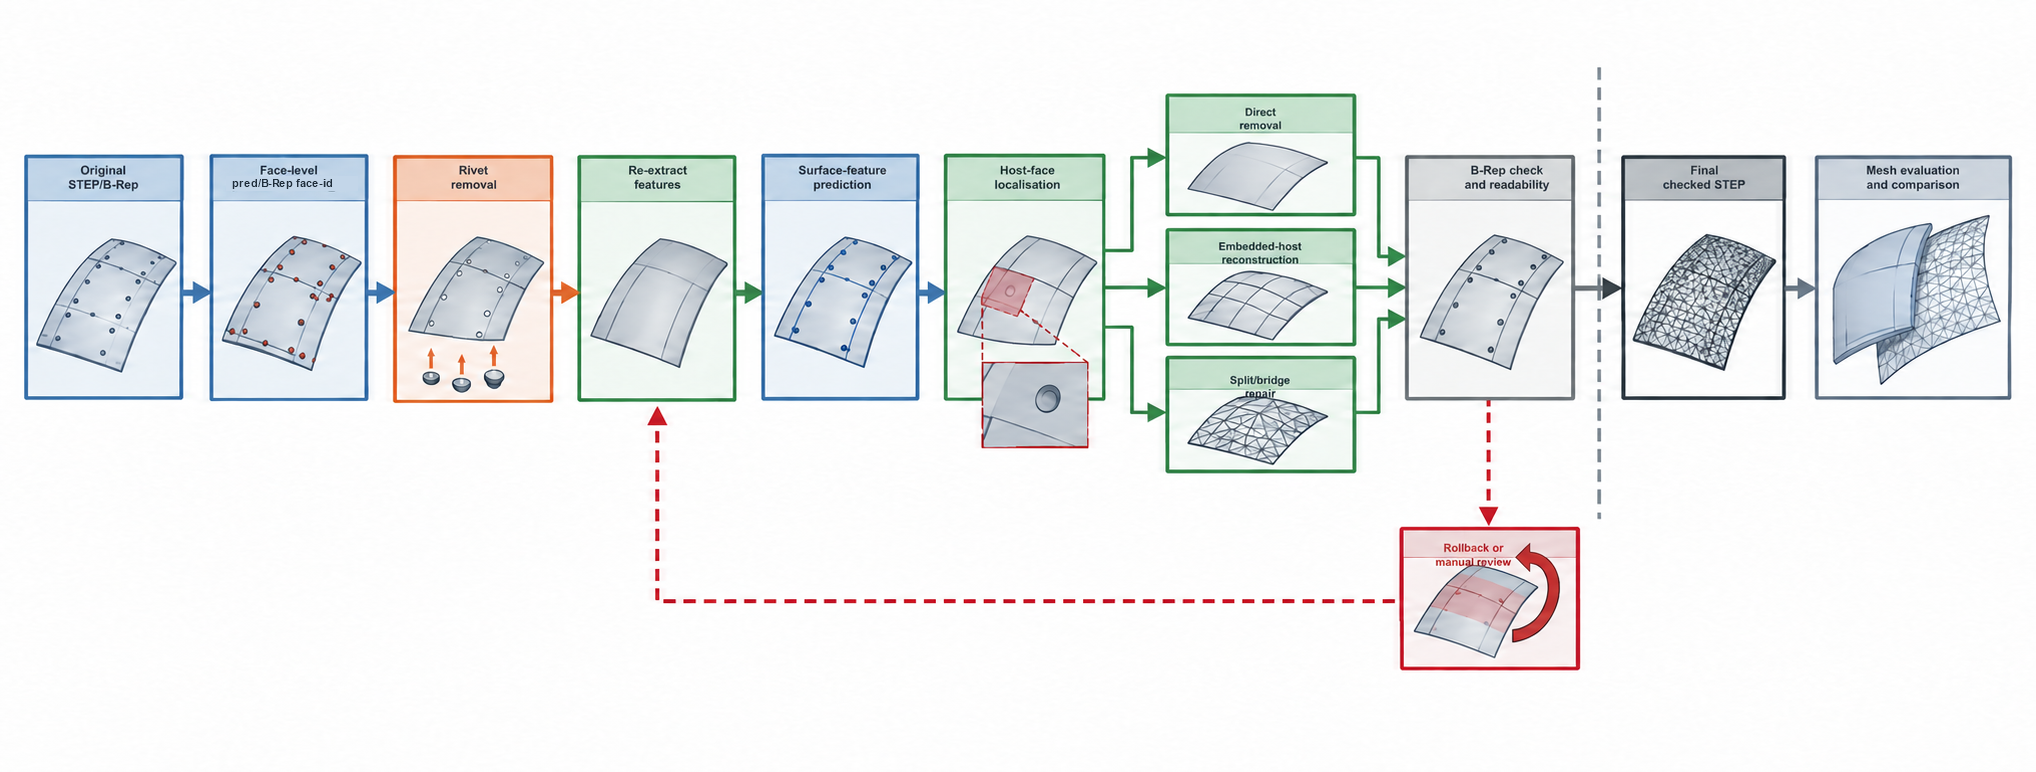
\includegraphics[width=0.95\linewidth]{figures/fig_feature_removal_reconstruction_protocol.png}
\caption{可追溯的特征去除与重建流程。第二阶段预测由去除铆钉后的中间模型生成，因此使用新的面标识符映射。}\label{fig:geometry_protocol}
\end{figure}

图~\ref{fig:geometry_protocol} 展示原始模型、中间模型和简化模型之间的处理关系。对于第二阶段的表面特征候选面，局部宿主关系决定受影响区域需要去除、重建还是修复。

图~\ref{fig:face_identifier_operation_link} 单独说明面标识符的作用。预测记录之所以可用于操作，是因为其面标识符能在相应 B-Rep 模型状态中定位到某一个具体面。操作改变拓扑后，下一次预测基于重新提取的中间模型生成，并使用新的标识符映射。

\begin{figure}[!ht]
\centering
\resizebox{0.95\linewidth}{!}{%
\begin{tikzpicture}[
  callout/.style={-{Latex[length=2mm]}, line width=.65pt, draw=black!65},
  record/.style={font=\sffamily\scriptsize, align=left, text=black!82}
]
  \node[inner sep=0pt] (original) at (0,29mm) {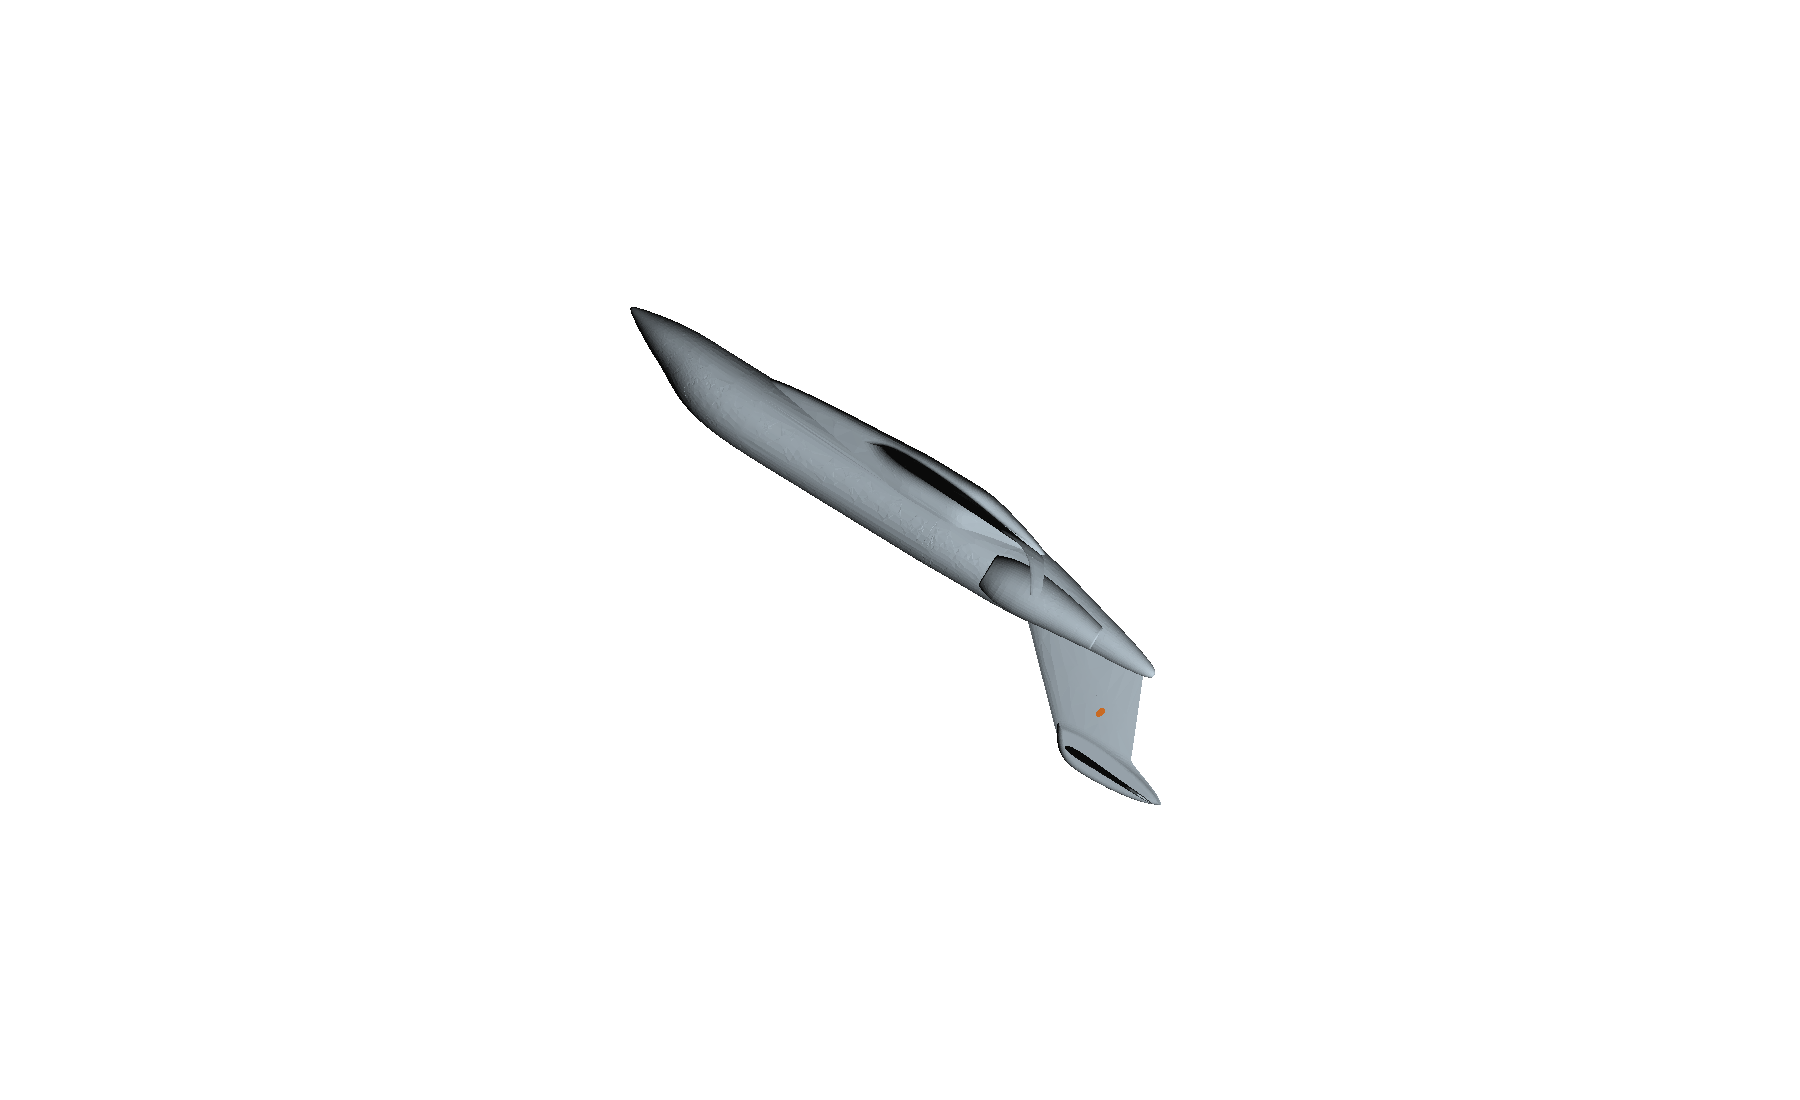
\includegraphics[width=52mm,trim=400 190 400 190,clip]{figures/gulfstream_sequence_figure5_original_target.png}};
  \node[inner sep=0pt] (originaldetail) at (62mm,29mm) {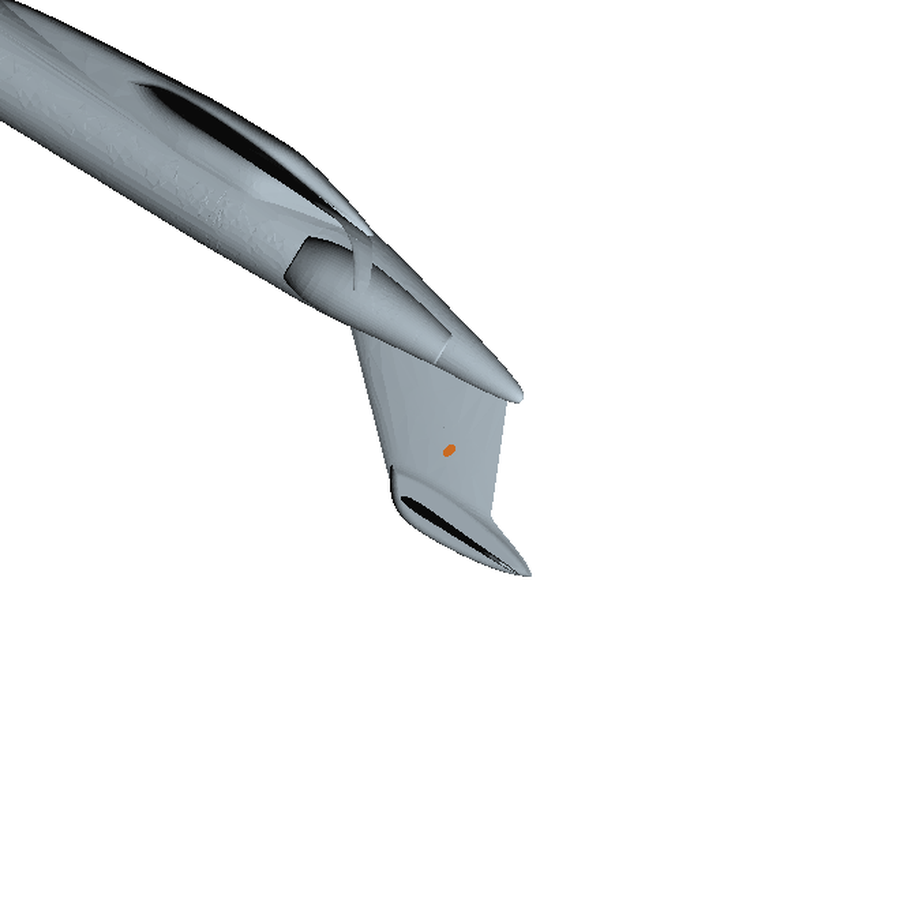
\includegraphics[width=30mm]{figures/gulfstream_sequence_figure5_original_target_detail.png}};
  \node[font=\sffamily\small\bfseries, anchor=south] at (original.north) {(A) 原始 B-Rep 模型};
  \node[font=\sffamily\scriptsize\bfseries, text=orange!80!black, anchor=south] at (originaldetail.north) {局部视图：面 $F_i$};
  \draw[blue!65!black, line width=.85pt] ($(original.center)+(10.5mm,-8.5mm)$) circle [radius=3mm];
  \draw[callout] ($(original.center)+(13mm,-8.5mm)$) to[out=0,in=180] (originaldetail.west);
  \node[record, anchor=west] at (84mm,37mm) {\textcolor{blue!65!black}{\textbf{预测记录}}\\状态：原始模型\\\textbf{面标识符：$F_i$}};
  \node[record, anchor=west] at (84mm,19mm) {\textcolor{teal!65!black}{\textbf{CAD 操作}}\\去除所选面};

  \draw[densely dashed, line width=.5pt, orange!85!black] (-30mm,0) -- (122mm,0);
  \node[fill=white, inner sep=2pt, font=\sffamily\scriptsize, text=orange!85!black, align=center] at (46mm,0) {拓扑改变；重新建立面编号};

  \node[inner sep=0pt] (intermediate) at (0,-31mm) {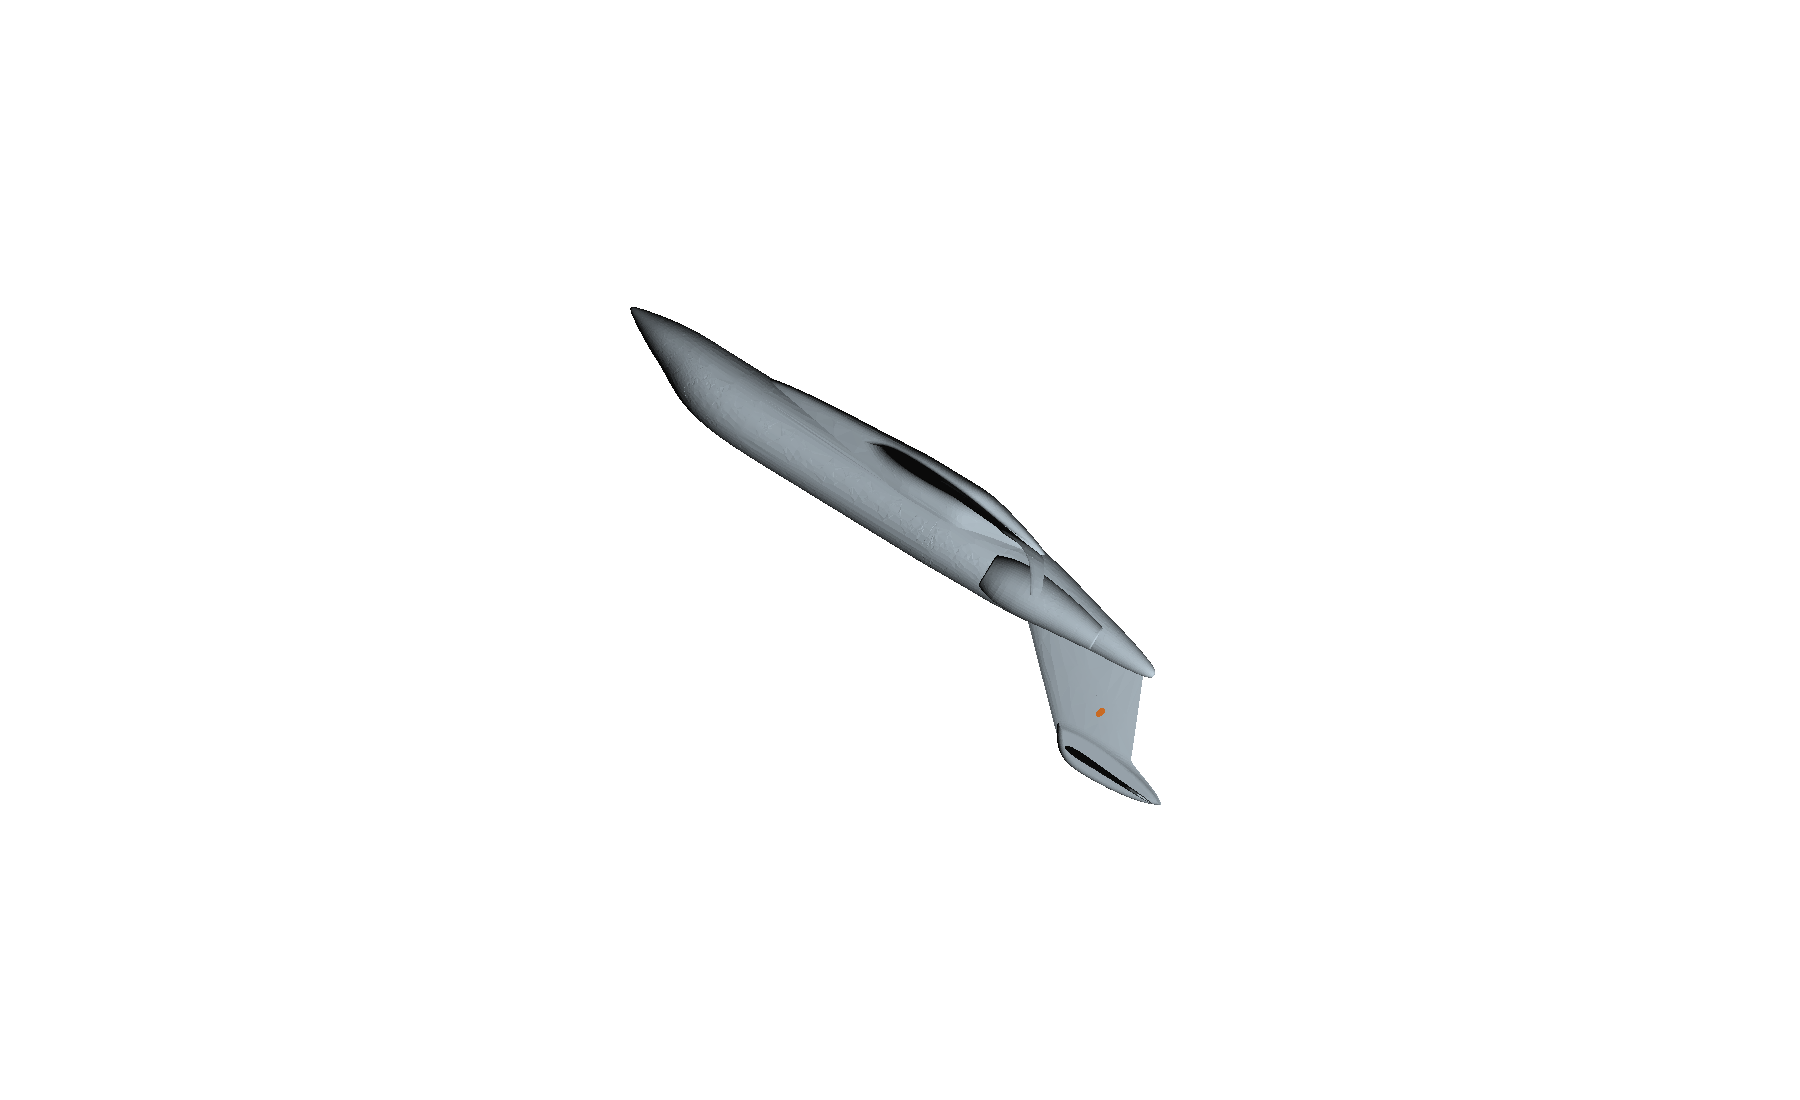
\includegraphics[width=52mm,trim=400 190 400 190,clip]{figures/gulfstream_sequence_figure5_intermediate_target.png}};
  \node[inner sep=0pt] (intermediatedetail) at (62mm,-31mm) {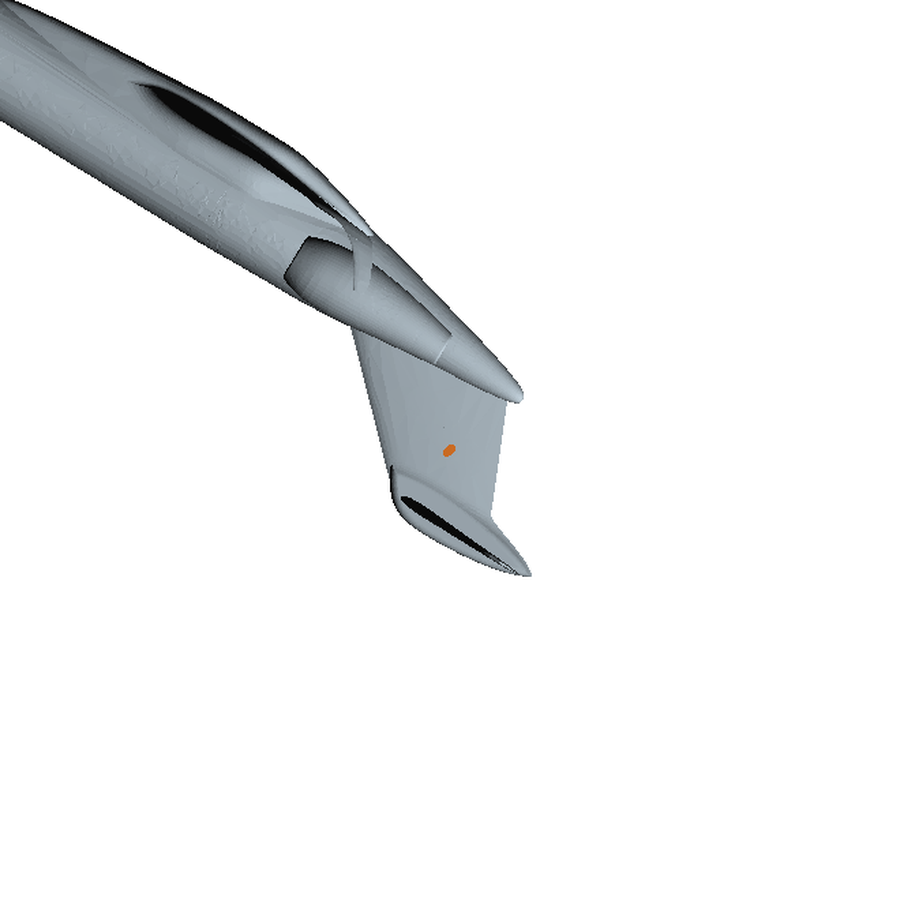
\includegraphics[width=30mm]{figures/gulfstream_sequence_figure5_intermediate_target_detail.png}};
  \node[font=\sffamily\small\bfseries, anchor=south] at (intermediate.north) {(B) 重新提取的中间模型};
  \node[font=\sffamily\scriptsize\bfseries, text=orange!80!black, anchor=south] at (intermediatedetail.north) {局部视图：面 $F'_j$};
  \draw[blue!65!black, line width=.85pt] ($(intermediate.center)+(10.5mm,-8.5mm)$) circle [radius=3mm];
  \draw[callout] ($(intermediate.center)+(13mm,-8.5mm)$) to[out=0,in=180] (intermediatedetail.west);
  \node[record, anchor=west] at (84mm,-23mm) {\textcolor{blue!65!black}{\textbf{预测记录}}\\状态：中间模型\\\textbf{面标识符：$F'_j$}};
  \node[record, anchor=west] at (84mm,-41mm) {\textcolor{teal!65!black}{\textbf{CAD 操作}}\\重建局部区域};
\end{tikzpicture}%
}
\caption{面标识符连接预测记录与具体 CAD 操作。每个高亮面均在完整 B-Rep 模型和局部视图中显示。对于图示操作，预测记录指定的是某一个面，而非全部候选面。$F_i$ 仅属于原始模型；拓扑变化后，$F'_j$ 属于重新提取的中间模型及另一套面映射。}\label{fig:face_identifier_operation_link}
\end{figure}

对每一对原始与简化模型，两个端点均使用相同的 OpenCASCADE 表面网格生成器，相对线性偏差为 0.0005，角度偏差为 0.5 rad \parencite{occt_mesh_2026}。每个端点重复运行五次，并取生成时间的中位数。表~\ref{tab:geometry_protocol} 列出网格规模和计时指标。这些指标均不能检验有限元精度或物理响应等价性。

对于网格生成后的基线方法，首先使用相同 OpenCASCADE 设置为原始 B-Rep 生成网格，再通过二次误差度量（QEM）边折叠进行简化 \parencite{garland1997qem}。每个模型的 QEM 目标是 B-Rep 处理路线得到的最终三角形数量。实现采用 \texttt{fast-simplification} 0.2.0，聚合因子为 7.0，并关闭边界保留 \parencite{fast_simplification_2026}。报告的基线计时组件为原始 B-Rep 网格生成时间中位数，加上五次 QEM 核心运行时间的中位数；不包含网格提取和数组转换、文件输入输出、识别、候选筛选及 CAD 操作。因此，这是一项匹配三角形规模的计时组件比较，而非完整流程耗时比较。

\begin{table}[!ht]
\centering
\small
\caption{原始与简化模型配对的表面网格测量方案。}\label{tab:geometry_protocol}
\begin{tabular}{p{0.32\linewidth}p{0.58\linewidth}}
\toprule
项目 & 设置或记录量 \\
\midrule
表面网格生成器 & OpenCASCADE 表面网格生成器 \\
相对线性偏差 & 0.0005 \\
角度偏差 & 0.5 rad \\
重复生成 & 每个模型运行五次，记录生成时间中位数 \\
网格规模 & 节点数与三角形数 \\
运行环境 & Windows 10 Pro 25H2；Intel Core i7-14700KF；NVIDIA GeForce RTX 4060（8~GB）；Python 3.10.20、OpenCASCADE 7.9.0 和 PyTorch 2.12.1+cu130 \\
\bottomrule
\end{tabular}
\end{table}

这些配对模型支持在固定网格参数下比较 CAD 面数和表面网格规模。去除是否完整、重建是否成功、几何保真程度以及物理响应是否等价，仍需额外证据。

\subsection{数据标注与训练方案}\label{sec:data_training}

\subsubsection{标注约定与模型级划分}\label{sec:data_partition}

标注记录保留每个原始面的面标识符及来源类别。铆钉面标为\textit{铆钉}，贴花面和窗户面共同标为\textit{表面特征}，其余面标为\textit{背景}。面标识符使每个标签在训练或评估前都能与相应 B-Rep 模型核对。

同一架飞机的全部面保留在同一数据划分中，以避免同机面及其局部邻接关系跨训练集和测试集重叠 \parencite{kapoor2023leakage}。模型参数和归一化统计量由训练集计算。完整测试集使用保存的特征顺序、统计量、类别映射和判定阈值处理，不用于更新本文报告的模型检查点。表~\ref{tab:data_composition} 给出面级指标对应的训练集与测试集构成。

\begin{table}[!ht]
\centering
\small
\caption{训练集与测试集的面级构成。百分比按各行总数计算。}\label{tab:data_composition}
\begin{tabular}{lrrrr}
\toprule
数据划分 & B-Rep 面总数 & 背景 & 铆钉 & 表面特征 \\
\midrule
训练集 & 48,095 & 44,716 (92.97\%) & 653 (1.36\%) & 2,726 (5.67\%) \\
测试集 & 34,162 & 33,073 (96.81\%) & 346 (1.01\%) & 743 (2.18\%) \\
\bottomrule
\end{tabular}
\end{table}

\subsubsection{训练配置与可复现性}\label{sec:training_configuration}

每架飞机由一个面图表示。训练集归一化统计量、特征顺序、类别映射、网络配置和判定阈值随检查点一同保存，并在推理中复用，使报告的训练集和测试集采用一致的预处理及预测规则。

报告的检查点使用表~\ref{tab:node_feature_contract} 所列的 48 个节点字段；其中八个曲面类型指示字段，是训练特征约定中出现的曲面类型的独热编码。图还保存六个边属性：边类型、面积比、邻面曲面类型、共享边界长度，以及二面角的均值和标准差。

\begin{table}[!ht]
\centering
\scriptsize
\caption{与报告的检查点一同保存的 48 个节点特征字段。字段名与实现保持一致。}\label{tab:node_feature_contract}
\begin{tabular}{p{0.25\linewidth}p{0.67\linewidth}}
\toprule
分组 & 字段 \\
\midrule
面几何与拓扑（24） & relativeArea, normalizedTrimmedArea, normalizedPerimeter, compactness, normalizedMeanCurvature, normalizedRadius, has\_radius, numWires, innerWireCount, normalizedMinInnerWireLength, normalizedMaxInnerWireLength, numEdges, normalizedNeighborAreaMean, normalizedNeighborAreaMax, areaToNeighborMean, areaToNeighborMax, neighborPlaneCount, neighborCylinderCount, neighborCurvedCount, convexEdgeCount, concaveEdgeCount, smoothEdgeCount, convexEdgeRatio, concaveEdgeRatio \\
附着与边界关系（11） & logNormalizedTrimmedArea, logNormalizedPerimeter, logAreaToNeighborMean, logAreaToNeighborMax, sameSurfaceNeighborRatio, smoothSameSurfaceNeighborRatio, smoothSameSurfaceBoundaryRatio, smoothSameSurfaceAreaContrast, hasLargerSmoothSameSurfaceNeighbor, uniqueNeighborToEdgeRatio, sharedBoundaryRatio \\
邻面法向关系（3） & normalNeighborDotMean, normalNeighborDotMin, normalNeighborDotMax \\
模型相对位置（2） & axisPositionAbs, radialDistance \\
曲面类型（8） & surfaceType\_0, surfaceType\_1, surfaceType\_2, surfaceType\_3, surfaceType\_4, surfaceType\_6, surfaceType\_7, surfaceType\_8 \\
\bottomrule
\end{tabular}
\end{table}

报告的训练运行使用 AdamW：初始学习率为 0.005，dropout 为 0.2，权重衰减为 $10^{-4}$，focal loss 的 $\gamma=2.0$，随机种子为 123；以批量大小 1 在完整飞机图上训练 50 个 epoch。AdamW 将权重衰减与自适应梯度更新解耦 \parencite{loshchilov2019adamw}。模型权重与训练集统计量作为配套的检查点文件保存。

\section{实验结果}\label{sec:results}

本节报告面级识别结果、可追溯的 CAD 处理输出，以及简化前后的表面网格比较。识别结果按面标识符将预测与真实标签对齐。CAD 表格记录各处理阶段的输入；候选面数量和可视化示例不用于衡量操作层面的完整性。

\subsection{面级识别与背景面风险分析}\label{sec:e1_results}

本文在完整测试集的全部 34,162 个面上评估既定模型检查点。每个模型的预测文件和真实标签文件均按面标识符对齐，因此类别指标与逐机错误数针对同一批面。由于缺少逐 epoch 的历史记录，报告数值表征的是所保存检查点的表现，而非训练收敛过程。

对每个类别，精确率（$P$）表示预测为该类的面中预测正确的比例，召回率（$R$）表示该类真实面中被找回的比例。F1 是两者的调和平均数，$F1 = 2PR/(P+R)$，用于概括误报候选面与漏检目标面之间的平衡。

完整测试集上，铆钉与表面特征的 F1 分数分别为 0.9312 和 0.8091（表~\ref{tab:e1_class_metrics}）。总体准确率为 0.9900，背景类 F1 为 0.9949。铆钉的精确率和召回率分别为 0.9436 和 0.9191；表面特征的精确率和召回率分别为 0.7841 和 0.8358。这些类别级指标补充了受背景面数量主导的总体准确率，并显示目标漏检与候选面误报之间仍存在权衡。

\begin{table}[!ht]
\centering
\small
\caption{完整测试集（34,162 个 B-Rep 面）的汇总面级识别结果。}\label{tab:e1_class_metrics}
\begin{tabular}{lrrrrr}
\toprule
类别 & 真实面数 & 精确率 & 召回率 & F1 & IoU \\
\midrule
背景 & 33,073 & 0.9955 & 0.9943 & 0.9949 & 0.9898 \\
铆钉 & 346 & 0.9436 & 0.9191 & 0.9312 & 0.8712 \\
表面特征 & 743 & 0.7841 & 0.8358 & 0.8091 & 0.6794 \\
\bottomrule
\end{tabular}
\end{table}

完整测试集中，背景面误报的分布并不均匀（表~\ref{tab:e1_risk}）。在 190 个被预测为目标类的背景面中，Air Plane Idea A 占 82 个，而 109 standard E-1 仅有 6 个。仅凭数量不足以反映几何风险：在报告的背景面误报中，Airbus 的最大相对面积最高（$8.80831\times10^{-2}$）。同时报告数量和面积，有助于区分频繁的局部误报与发生在较大背景面上的单次误报。

\begin{table}[!ht]
\centering
\small
\caption{完整测试集的逐机背景面误报风险。最大相对面积是被预测为任一目标类的背景面中的最大值。}\label{tab:e1_risk}
\begin{tabular}{lrrrrrr}
\toprule
模型 & 面数 & 准确率 & $B\rightarrow R$ & $B\rightarrow S$ & 合计 & 最大相对面积 \\
\midrule
109 standard E-1 & 1,244 & 0.9936 & 0 & 6 & 6 & $9.95\times10^{-7}$ \\
DC-10 & 287 & 0.9477 & 0 & 2 & 2 & $9.61987\times10^{-5}$ \\
747-400 & 1,432 & 0.9874 & 10 & 0 & 10 & $2.56619\times10^{-8}$ \\
AULIRA 2 & 370 & 0.9459 & 0 & 16 & 16 & $6.91349\times10^{-6}$ \\
Air Plane Idea A & 27,366 & 0.9970 & 9 & 73 & 82 & $2.20926\times10^{-4}$ \\
Airbus & 1,775 & 0.9104 & 0 & 52 & 52 & $8.80831\times10^{-2}$ \\
Airplane body & 708 & 0.9760 & 0 & 10 & 10 & $7.21426\times10^{-4}$ \\
Cessna Citation 2 & 312 & 0.9712 & 0 & 4 & 4 & $5.58992\times10^{-4}$ \\
Gulfstream G280 v17 & 668 & 0.9820 & 0 & 8 & 8 & $2.67640\times10^{-3}$ \\
\bottomrule
\end{tabular}
\end{table}

汇总的类别分数无法显示每架飞机包含多少目标面、漏检了多少目标面。表~\ref{tab:e1_per_aircraft_targets} 根据上述相同的预测--真实标签配对，报告这些数量及各机内部的 F1 分数。漏检目标面是指被归入其他类别的真实铆钉面或表面特征面。

\begin{table}[!ht]
\centering
\small
\caption{完整测试集的逐机目标类结果。“真实面数”指该类真实面的数量，“漏检”指被判为其他类的数量。Air Plane Idea A 没有真实铆钉面，因此该机的铆钉 F1 以短横线表示。}\label{tab:e1_per_aircraft_targets}
\resizebox{\linewidth}{!}{%
\begin{tabular}{lrrrrrr}
\toprule
 & \multicolumn{3}{c}{铆钉} & \multicolumn{3}{c}{表面特征} \\
\cmidrule(lr){2-4}\cmidrule(lr){5-7}
模型 & 真实面数 & 漏检 & F1 & 真实面数 & 漏检 & F1 \\
\midrule
109 standard E-1 & 26 & 2 & 0.9600 & 1 & 0 & 0.2500 \\
DC-10 & 26 & 2 & 0.9600 & 119 & 11 & 0.9432 \\
747-400 & 20 & 2 & 0.7500 & 256 & 6 & 0.9881 \\
AULIRA 2 & 52 & 4 & 0.9600 & 10 & 0 & 0.5556 \\
Air Plane Idea A & 0 & 0 & -- & 88 & 0 & 0.7068 \\
Airbus & 52 & 4 & 0.9600 & 194 & 103 & 0.5401 \\
Airplane body & 58 & 6 & 0.9455 & 20 & 1 & 0.7755 \\
Cessna Citation 2 & 52 & 4 & 0.9600 & 19 & 1 & 0.8780 \\
Gulfstream G280 v17 & 60 & 4 & 0.9655 & 36 & 0 & 0.9000 \\
\midrule
完整测试集 & 346 & 28 & 0.9312 & 743 & 122 & 0.8091 \\
\bottomrule
\end{tabular}
}
\end{table}

\FloatBarrier

目标类结果因飞机而异。在漏检的 122 个表面特征面中，Airbus 占 103 个；747-400 的 256 个真实表面特征面中则有 6 个漏检。109 standard E-1 只有 1 个真实表面特征面，因此其 0.2500 的 F1 分数对少量错误预测尤为敏感。Air Plane Idea A 占 34,162 个测试面中的 27,366 个，但没有真实铆钉面。因此，汇总分数描述的是这一固定的九机测试集合，不能解释为每架飞机和每个类别上都同样稳定的表现。

\subsection{可追溯的 CAD 处理输出}\label{sec:e2_results}

\subsubsection{特征去除与重建}

第~\ref{sec:geometry_protocol} 节的分阶段方案先处理铆钉预测，再从中间模型重新提取特征，供表面特征处理使用。重新提取是必要的，因为第二阶段的面标识符属于中间模型，而不属于原始模型。表~\ref{tab:e2_results} 记录各处理案例的候选输入。其中，铆钉数量是在面级识别结果采用的附加平面区域检查之前统计的；表面特征数量对应中间模型。Air Plane Idea A 采用仅处理贴花的路线，不进行铆钉去除。

候选面数量差异较大，因为一个物理特征可能由多个 B-Rep 面表示，各源模型的面划分也不同。因此，表中报告的是操作输入，而非特征实例数量或去除成功率。

\begin{table}[!ht]
\centering
\small
\captionsetup{justification=raggedright,singlelinecheck=false}
\caption{提供给 CAD 处理的可追溯预测面输出。Air Plane Idea A 的短横线表示其仅处理贴花的路线不包含铆钉去除，并非铆钉分类结果。}\label{tab:e2_results}
\resizebox{\linewidth}{!}{%
\begin{tabular}{lrr}
\toprule
测试模型 & 预测铆钉面数 & 预测表面特征面数 \\
\midrule
109 standard E-1 & 26 & 27 \\
DC-10 & 26 & 110 \\
747-400 & 30 & 254 \\
AULIRA 2 & 52 & 100 \\
Air Plane Idea A & -- & 88 \\
Airbus & 52 & 960 \\
Airplane body & 58 & 53 \\
Cessna Citation 2 & 52 & 23 \\
Gulfstream G280 v17 & 60 & 50 \\
\bottomrule
\end{tabular}
}
\end{table}

处理输出在每个阶段均保留面标识符，因此可在相应的原始或中间 B-Rep 模型上检查。图~\ref{fig:e2_rivet_examples} 和图~\ref{fig:e2_window_examples} 通过铆钉、贴花和窗户类区域的示例展示这种对应关系。示例表明，流程能够产生与预测面关联的局部变化，但尚不能证明操作层面的完整性。

\begin{figure}[!ht]
\centering
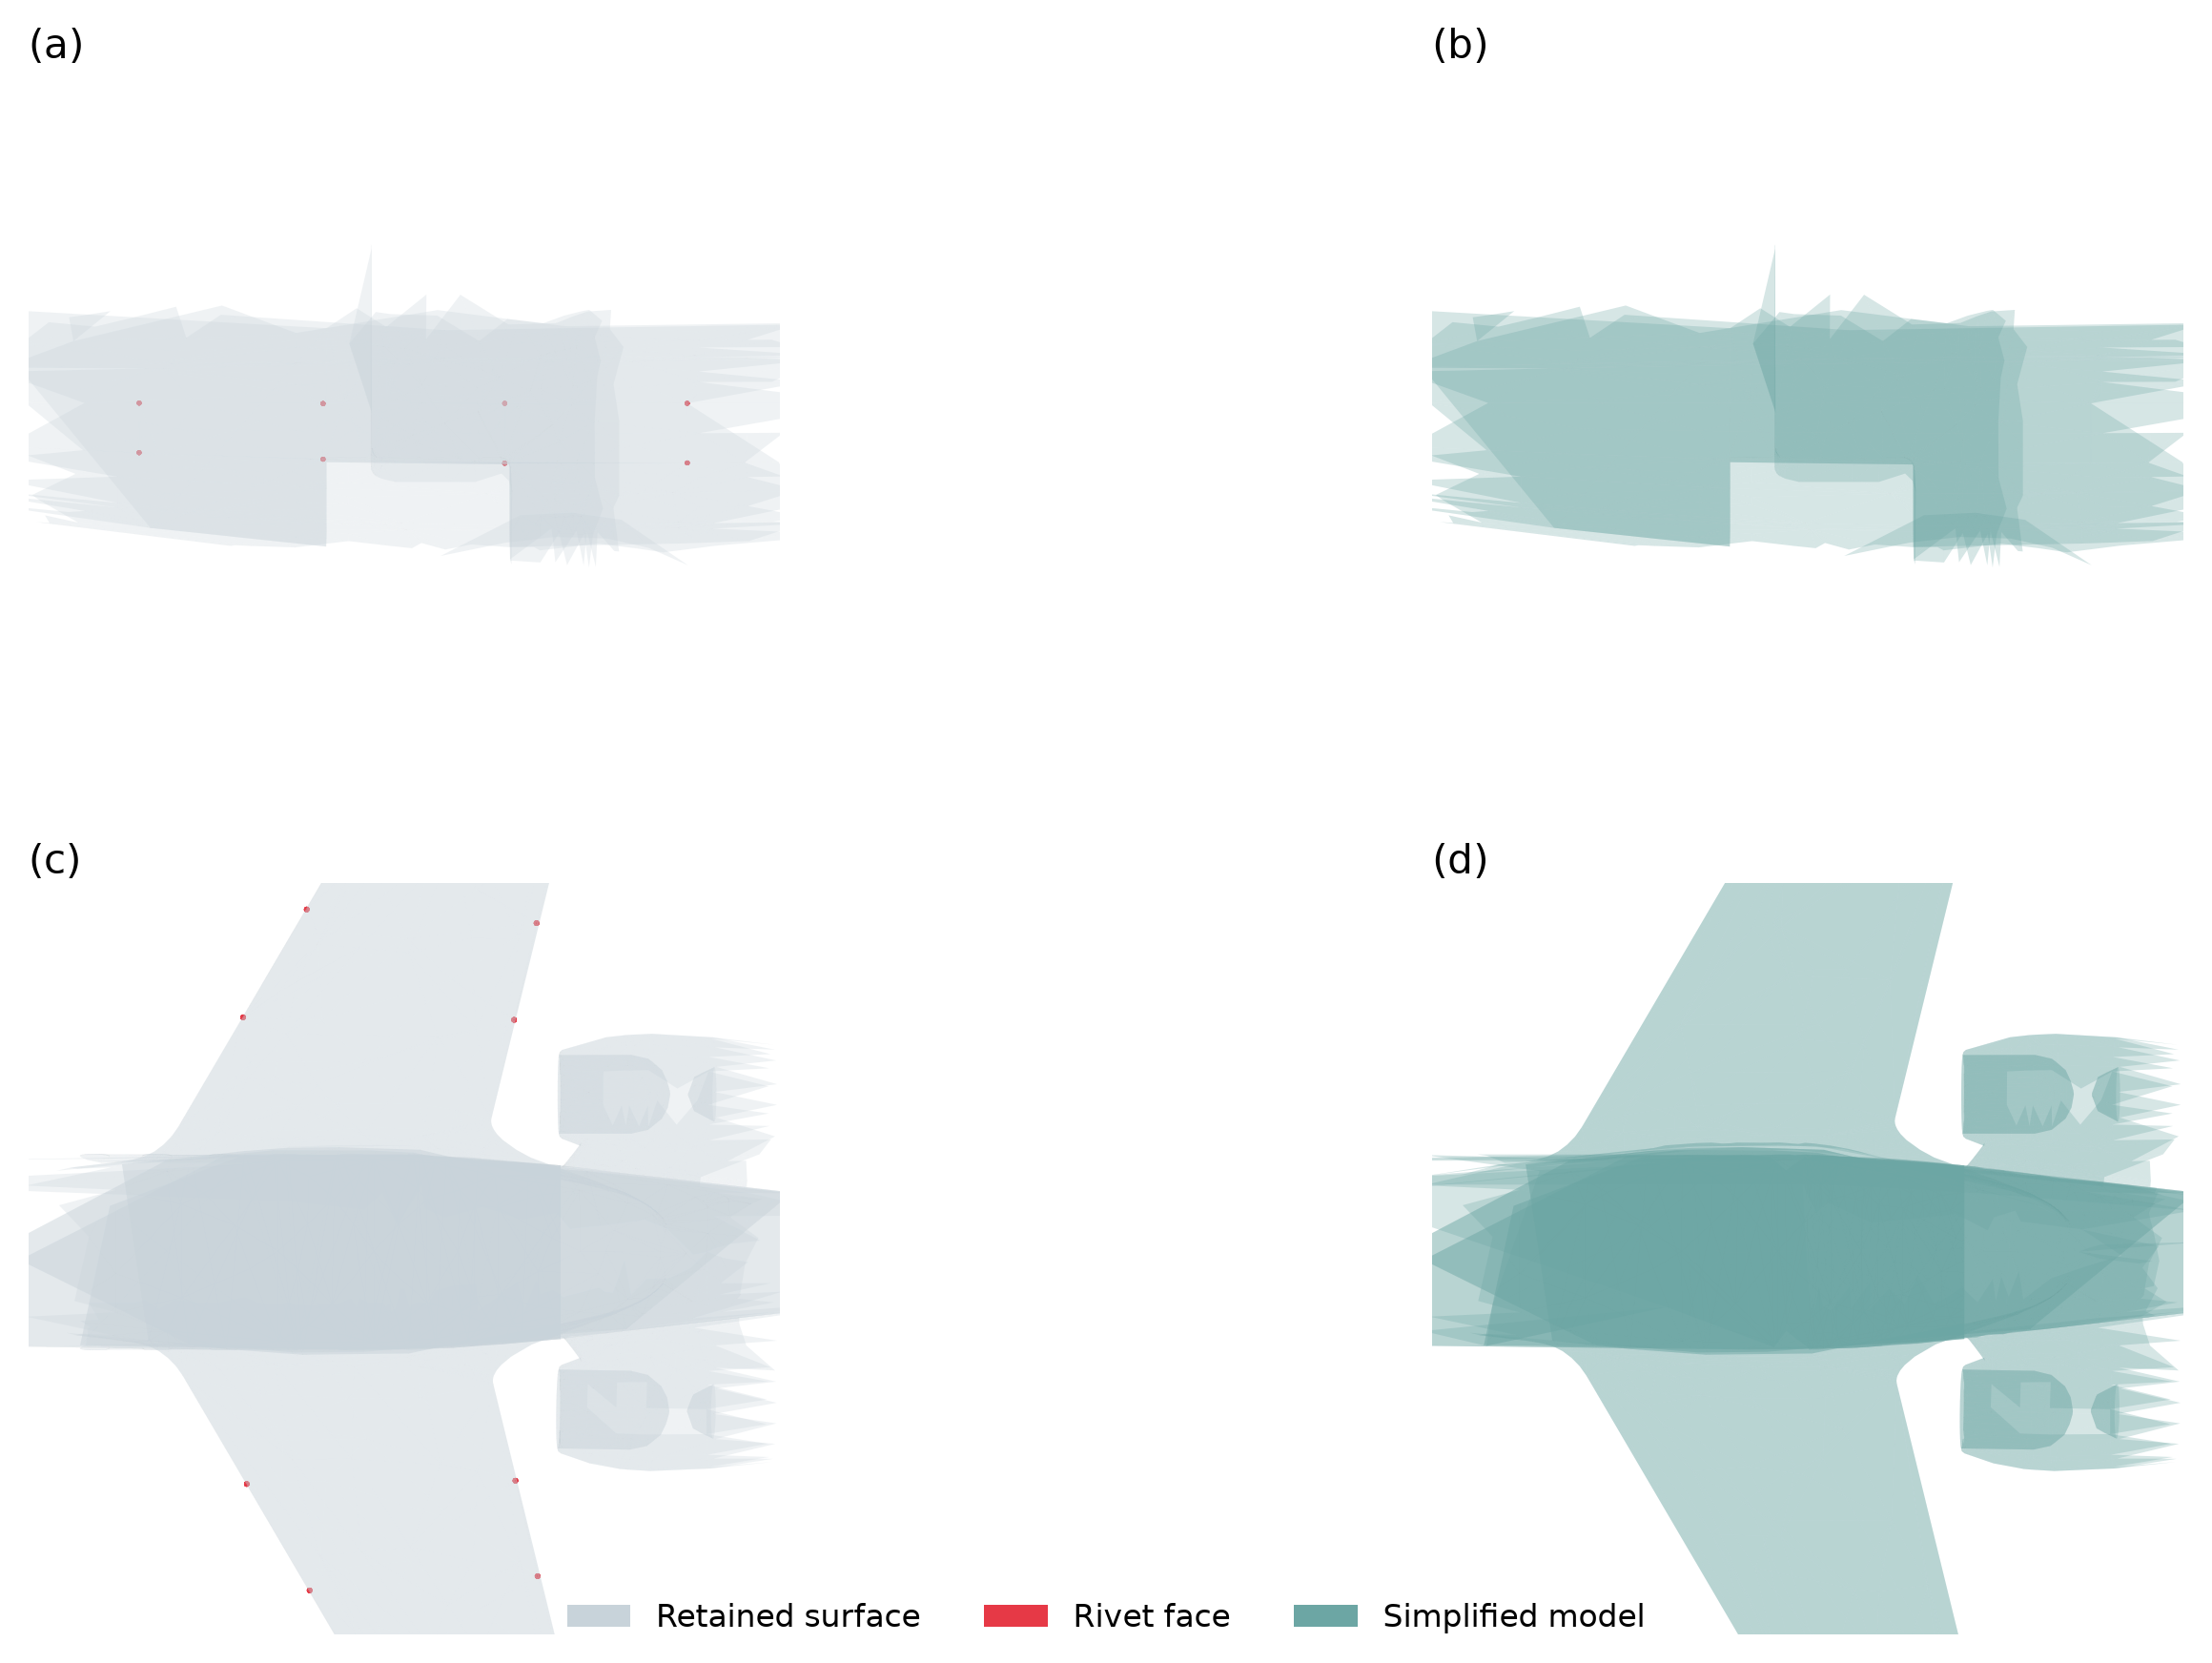
\includegraphics[width=0.92\linewidth]{figures/e2_rivet_before_after.png}
\caption{铆钉去除对比。（a、b）模型 109 去除前后；（c、d）Gulfstream G280 v17 使用流程预测结果去除前后。红色表示铆钉面，灰色表示保留的表面，蓝绿色表示简化模型。}\label{fig:e2_rivet_examples}
\end{figure}

\clearpage
\begin{figure}[!ht]
\centering
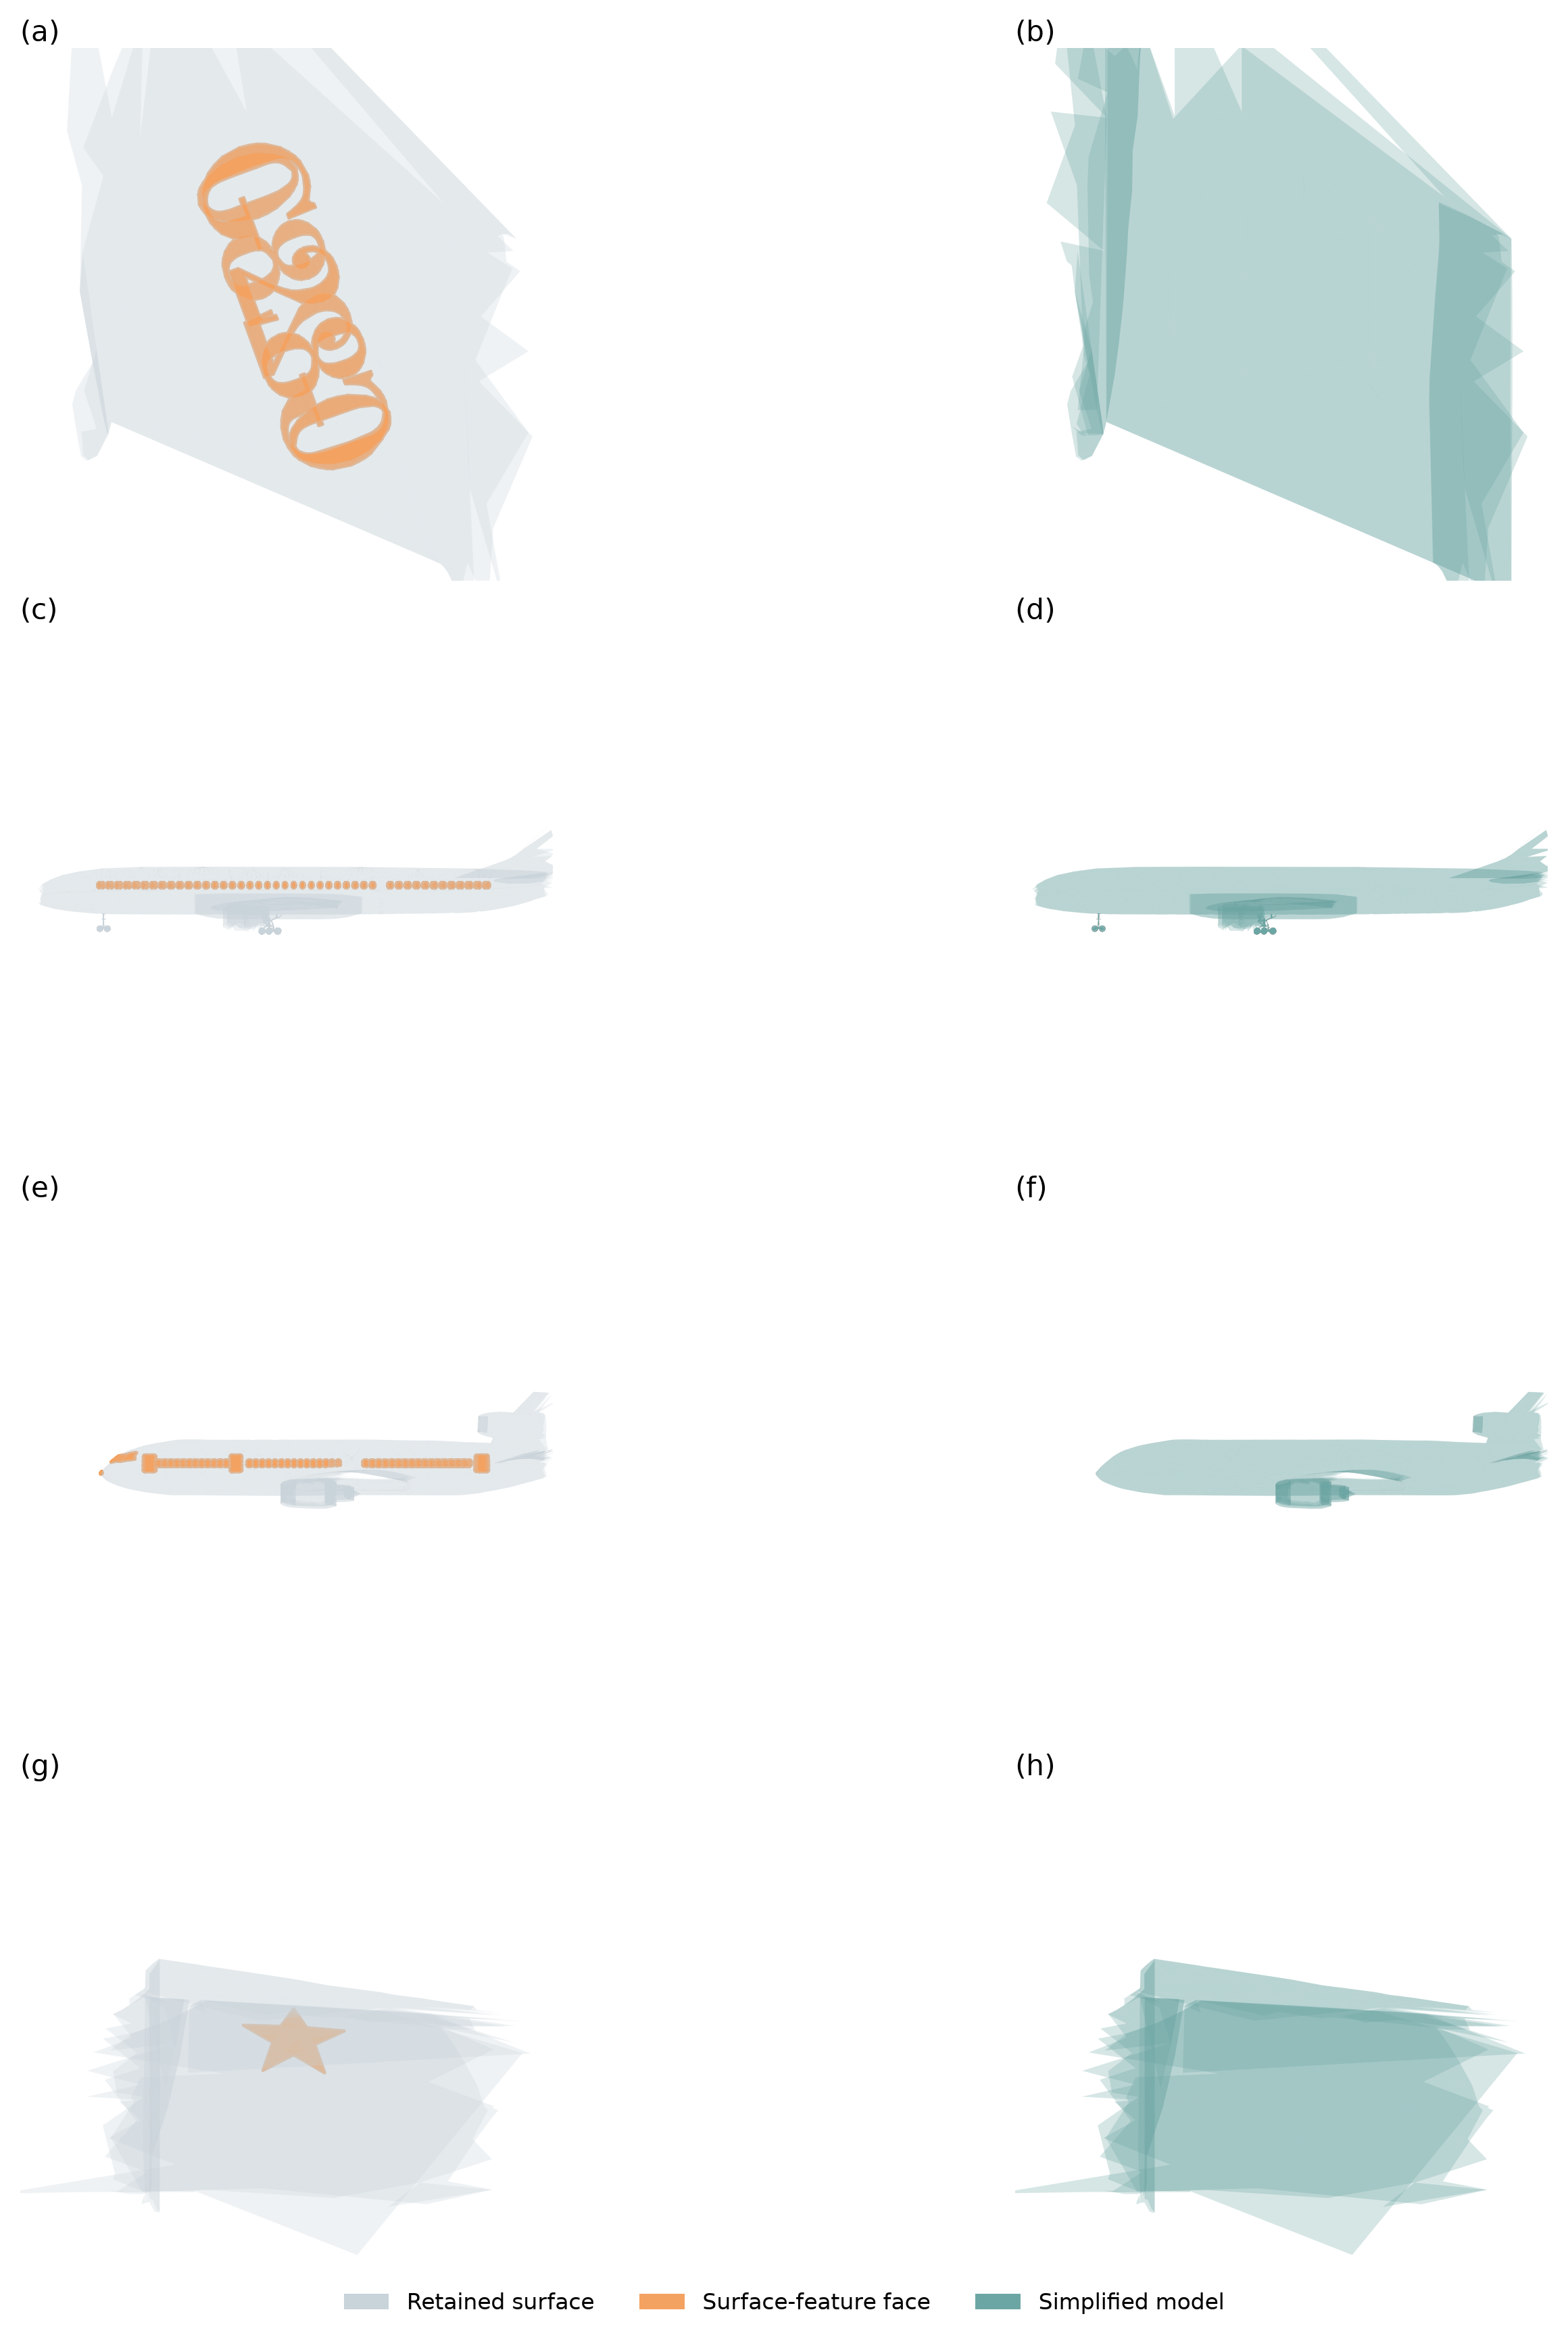
\includegraphics[width=0.92\linewidth]{figures/e2_window_before_after.png}
\caption{侧视图中的表面特征去除对比。（a、b）Gulfstream G280 v17 的贴花区域，（c、d）Air Plane Idea A，（e、f）DC-10，以及（g、h）模型 109 的星形贴花区域，分别显示去除前后。橙色表示原始模型上预测为表面特征的面，灰色表示保留的表面，蓝绿色表示简化模型。}\label{fig:e2_window_examples}
\end{figure}

\subsubsection{原始与简化模型的表面网格比较}\label{sec:e3_results}

使用第~\ref{sec:geometry_protocol} 节给出的 OpenCASCADE 设置，对每组原始与简化模型生成网格。每个端点重复五次，并以生成时间中位数进行组内比较。固定设置使同一对模型的测量可比，但不能证明网格适合某一特定分析任务 \parencite{thakur2009cad_simplification}。

图~\ref{fig:e3_mesh_schematic} 通过两个示意性的飞机表面说明比较内容：原始模型的小特征周围网格更密，局部去除与重建后的机身表面更连续。该图用于解释；全部九对模型的测量结果见表~\ref{tab:e3_mesh}。

\begin{figure}[!ht]
\centering
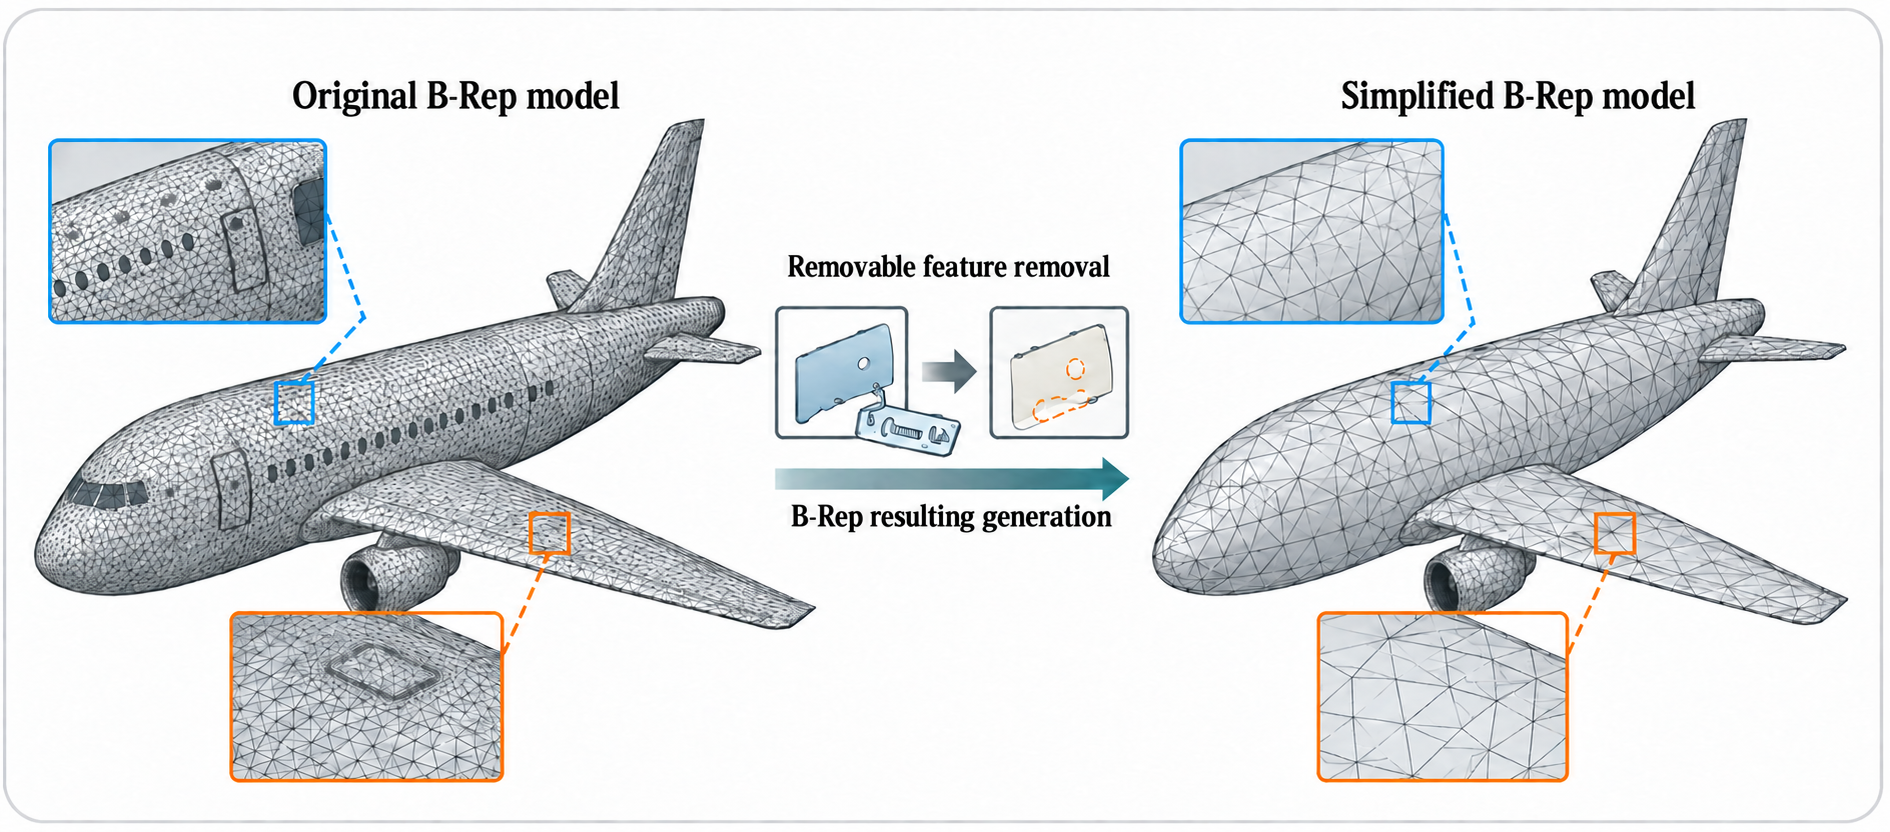
\includegraphics[width=0.98\linewidth]{figures/fig_original_simplified_mesh_comparison_v4.png}
\caption{局部特征去除与曲面重建前后的示意性表面网格比较。为便于观察，网格显示在完整外表面上；定量结果见表~\ref{tab:e3_mesh}。}
\label{fig:e3_mesh_schematic}
\end{figure}

九对模型在简化后均表现出更少的 CAD 面、网格节点和表面三角形，以及更短的网格生成时间中位数（表~\ref{tab:e3_mesh}）。三角形数量减少 0.57\%--48.66\%，时间减少 2.49\%--58.29\%。两项指标并不成比例：Air Plane Idea A 的三角形数量减少 3.16\%，时间中位数减少 2.49\%；而 DC-10 的三角形数量减少 15.31\%，时间减少 57.40\%。因此，数据支持的是所述网格设置下的配对减少，不能把三角形数量变化固定换算为时间变化。面划分、处理结果和重建区域的差异都可能造成这种变化，但各自的作用尚未单独测量。

\begin{table}[!ht]
\centering
\caption{简化前后的表面网格规模及网格生成时间中位数。}\label{tab:e3_mesh}
\resizebox{\linewidth}{!}{%
\begin{tabular}{lrrrr}
\toprule
模型 & CAD 面数 & 节点数 & 三角形数 & 时间中位数（s） \\
\midrule
AULIRA 2 & 370 $\rightarrow$ 136 & 16,178 $\rightarrow$ 7,824 & 24,519 $\rightarrow$ 12,589 ($-48.66\%$) & 0.1378 $\rightarrow$ 0.0735 ($-46.65\%$) \\
747-400 & 1,432 $\rightarrow$ 1,132 & 59,108 $\rightarrow$ 37,195 & 76,017 $\rightarrow$ 48,959 ($-35.59\%$) & 0.6227 $\rightarrow$ 0.3373 ($-45.84\%$) \\
Airbus & 1,775 $\rightarrow$ 686 & 69,556 $\rightarrow$ 43,042 & 95,610 $\rightarrow$ 63,505 ($-33.58\%$) & 0.6107 $\rightarrow$ 0.2547 ($-58.29\%$) \\
Gulfstream G280 v17 & 668 $\rightarrow$ 277 & 15,858 $\rightarrow$ 10,244 & 17,941 $\rightarrow$ 14,378 ($-19.86\%$) & 0.1816 $\rightarrow$ 0.1035 ($-43.00\%$) \\
Airplane body & 708 $\rightarrow$ 450 & 34,721 $\rightarrow$ 27,114 & 51,605 $\rightarrow$ 42,401 ($-17.84\%$) & 0.2788 $\rightarrow$ 0.1925 ($-30.95\%$) \\
DC-10 & 287 $\rightarrow$ 170 & 27,041 $\rightarrow$ 20,608 & 41,914 $\rightarrow$ 35,496 ($-15.31\%$) & 0.2215 $\rightarrow$ 0.0943 ($-57.40\%$) \\
Cessna Citation 2 & 312 $\rightarrow$ 231 & 13,756 $\rightarrow$ 12,838 & 19,696 $\rightarrow$ 19,037 ($-3.35\%$) & 0.0923 $\rightarrow$ 0.0725 ($-21.54\%$) \\
Air Plane Idea A & 27,366 $\rightarrow$ 27,278 & 443,054 $\rightarrow$ 433,184 & 438,769 $\rightarrow$ 424,893 ($-3.16\%$) & 3.6364 $\rightarrow$ 3.5458 ($-2.49\%$) \\
109 standard E-1 & 1,244 $\rightarrow$ 986 & 47,808 $\rightarrow$ 46,811 & 58,692 $\rightarrow$ 58,357 ($-0.57\%$) & 0.4108 $\rightarrow$ 0.3410 ($-16.98\%$) \\
\bottomrule
\end{tabular}
}
\end{table}

为在匹配输出规模的条件下与网格生成后的简化方法比较，本文使用 QEM 边折叠简化原始 B-Rep 网格。每对模型的 QEM 目标是 B-Rep 处理路线的最终三角形数量。表~\ref{tab:qem_matched_time} 按上述计时口径报告两个计时组件。

\begin{table}[!ht]
\centering
\caption{与 QEM 进行匹配三角形规模的计时组件比较。基线为原始 B-Rep 网格生成加 QEM 核心运行，本文组件为几何处理后的最终网格生成。相对差异根据未四舍五入的时间计算。}\label{tab:qem_matched_time}
\resizebox{\linewidth}{!}{%
\begin{tabular}{lrrrr}
\toprule
模型 & QEM 三角形数 & 最终网格生成（s） & 原始网格生成 + QEM 核心（s） & 相对差异（\%） \\
\midrule
AULIRA 2 & 12,588 & 0.0735 & 0.1481 & 50.34 \\
747-400 & 48,959 & 0.3373 & 0.6497 & 48.08 \\
Airbus & 63,504 & 0.2547 & 0.6376 & 60.05 \\
Gulfstream G280 v17 & 14,378 & 0.1035 & 0.1859 & 44.33 \\
Airplane body & 42,400 & 0.1925 & 0.2961 & 34.98 \\
DC-10 & 35,496 & 0.0943 & 0.2310 & 59.16 \\
Cessna Citation 2 & 19,036 & 0.0725 & 0.0962 & 24.69 \\
Air Plane Idea A & 424,892 & 3.5458 & 3.8216 & 7.22 \\
109 standard E-1 & 58,356 & 0.3410 & 0.4204 & 18.88 \\
\bottomrule
\end{tabular}
}
\end{table}
\FloatBarrier

在匹配的三角形数量目标下，由于边折叠是离散操作，QEM 输出的三角形数等于目标值或比目标值少一个。九对模型中，B-Rep 处理后的最终网格生成组件均低于“原始网格生成加 QEM 核心”组件，相对差异为 7.22\%--60.05\%，中位数为 44.33\%。这一结果仅适用于所列计时组件，不比较两条路线的端到端处理时间、几何保真程度或网格质量。

\subsection{讨论与证据边界}\label{sec:experimental_boundaries}

面级评估表明，本文方法能够在所报告的完整飞机 B-Rep 测试集中识别铆钉面和表面特征面，两类 F1 分数分别为 0.9312 和 0.8091。导出的面标识符使预测能够在相应 B-Rep 模型上定位。分阶段处理案例提供了可追溯的候选输入；九对原始与简化模型在测试设置下具有更少的表面三角形和更短的网格生成时间中位数。这些记录没有量化单个 CAD 操作成功完成的数量。

在接受几何操作结果前，仍应检查预测。表~\ref{tab:e1_per_aircraft_targets} 显示，九架飞机的目标类真实面数和漏检面数差异明显，表面特征尤为如此；汇总 F1 并不意味着逐机表现都同样稳定。剩余背景面误报也因模型而异，表面特征分支的召回率高于精确率，因此候选表面特征中仍包含部分背景面。候选面数量是操作输入，不是特征实例数量或完成去除的数量。由于铆钉处理会改变面编号，第二阶段预测前需重新提取模型；其面标识符指向中间模型，而非原始模型。

在固定的 OpenCASCADE 参数下，表~\ref{tab:e3_mesh} 中各配对模型简化后的表面三角形数和网格生成时间中位数均更低。三角形数量与时间的变化并不成比例，说明单凭三角形数量不能确定网格生成时间。在匹配三角形数量目标时，按明确限定的计时口径，表~\ref{tab:qem_matched_time} 中的最终网格生成组件也低于原始网格生成加 QEM 核心组件。这些结果描述的是所述设置下 CAD 面数和网格规模的变化；它们不能证明端到端时间优势、几何保真、B-Rep 等价或分析响应保持。

\section{结论}
本文构建了完整飞机 B-Rep 模型中铆钉面和表面特征面的面级识别框架，并保留面标识符，使预测能够被定位为几何操作候选面。每个面及其共享边界关系被编码为图，两个类别专用 GNN 生成三类输出。每条导出预测均保留面标识符，从而将学习得到的标签与相应原始或中间模型上的可编辑 B-Rep 实体关联。

在包含 34,162 个面的完整测试集上，铆钉和表面特征的 F1 分数分别为 0.9312 和 0.8091。在相同网格设置下，所报告的原始与简化模型配对中，表面三角形数量减少 0.57\%--48.66\%，网格生成时间中位数减少 2.49\%--58.29\%。在匹配三角形数量目标下，B-Rep 处理后的最终网格生成组件比单独计时的“原始网格生成加 QEM 核心”组件低 7.22\%--60.05\%。面标识符使预测可被定位为 CAD 处理候选面；配对结果表明，测试模型的网格复杂度和网格生成时间均有所降低。这些结果支持可核查的 CAD 与网格准备过程，但未量化单条预测或单次操作的影响。本文没有评估求解器运行时间或工程响应。

现有证据尚不能证明方法可迁移至其他 CAD 来源、特征能够完整去除、端到端耗时优于 QEM、几何保真达到要求，或对下游 CAE 任务具有等价效果。候选面数量不是操作成功率。后续研究应评估外部 CAD 来源，记录每次去除和重建尝试的结果，采用匹配的质量标准与完整计时比较两条路线，通过重复的受控实验分离各组件的作用，并在明确载荷和边界条件下评估特定任务的 CAE 响应。只有完成这些工作，才能判断几何变化在何种分析目的下可被接受。

%--- Mandatory Section ---%
\section*{作者贡献}
原稿此处仍为作者贡献模板，要求按 NISO CRediT（贡献者角色分类法）列出所有作者的完整姓名与个人贡献，说明见 \url{https://credit.niso.org/}。原稿提供的示例为：

\noindent\textbf{Kunwoo Lee}：概念设计、方法、软件。\textbf{Shuming Gao}：数据整理、初稿撰写。\textbf{Sang Hun Lee}：可视化、调查研究。\textbf{Jami J. Shah}：指导。\textbf{Hiromasa Suzuki}：软件、验证。\textbf{Myung-Il Roh}：审阅与修改。

%-------------------------------------------
% Template acknowledgement statements disabled until author metadata is finalised.
%-------------------------------------------
\iffalse

%--- Mandatory Section ---%
\section*{Conflicts of interest}
The authors must declare conflicts of interest or state ``The authors declare no conflict of interest.'' Authors must identify and declare any personal circumstances or interests that may be perceived as inappropriately influencing the representation or interpretation of reported research results. A detailed definition of conflicts of interest is available at the following site: \url{https://academic.oup.com/journals/pages/authors/preparing_your_manuscript/ethics#conflict}.

%--- Section ---%
\section*{Funding}
Cite all funding for your research, providing the grant number and the funder name. An example statement is as follows: This work is supported in part by funds from the National Science Foundation (NSF: \# 1636933 and \# 1920920).

If the funder is listed in the \href{https://www.crossref.org/services/funder-registry/}{Crossref Funder Registry}, the funder name should appear exactly as it does in that database. Where grants were received by specific members of the author group, they should be identified by initials.

More information on funding agency requirements is available from the \href{https://academic.oup.com/pages/open-research/open-access/complying-with-funder-policies}{Oxford Academic funding-policy guidance}.

%--- Section ---%
\section*{Data availability}
The data availability statement should provide information on where and under what conditions the data directly supporting the publication can be accessed. Sample data availability statements are available at the following site: \url{https://academic.oup.com/pages/open-research/research-data#Data%20Availability%20Statements}.

%--- Section ---%
\section*{Acknowledgments}
The authors thank those people or institutions that have helped you in the preparation of the manuscript.


\fi

%-------------------------------------------
% References
%-------------------------------------------

% Print bibliography
\renewcommand*{\bibfont}{\small}
\printbibliography[title={参考文献}]





\end{document}
